\documentclass[twoside]{book}

% Packages required by doxygen
\usepackage{fixltx2e}
\usepackage{calc}
\usepackage{doxygen}
\usepackage[export]{adjustbox} % also loads graphicx
\usepackage{graphicx}
\usepackage[utf8]{inputenc}
\usepackage{makeidx}
\usepackage{multicol}
\usepackage{multirow}
\PassOptionsToPackage{warn}{textcomp}
\usepackage{textcomp}
\usepackage[nointegrals]{wasysym}
\usepackage[table]{xcolor}

% Font selection
\usepackage[T1]{fontenc}
\usepackage[scaled=.90]{helvet}
\usepackage{courier}
\usepackage{amssymb}
\usepackage{sectsty}
\renewcommand{\familydefault}{\sfdefault}
\allsectionsfont{%
  \fontseries{bc}\selectfont%
  \color{darkgray}%
}
\renewcommand{\DoxyLabelFont}{%
  \fontseries{bc}\selectfont%
  \color{darkgray}%
}
\newcommand{\+}{\discretionary{\mbox{\scriptsize$\hookleftarrow$}}{}{}}

% Page & text layout
\usepackage{geometry}
\geometry{%
  a4paper,%
  top=2.5cm,%
  bottom=2.5cm,%
  left=2.5cm,%
  right=2.5cm%
}
\tolerance=750
\hfuzz=15pt
\hbadness=750
\setlength{\emergencystretch}{15pt}
\setlength{\parindent}{0cm}
\setlength{\parskip}{3ex plus 2ex minus 2ex}
\makeatletter
\renewcommand{\paragraph}{%
  \@startsection{paragraph}{4}{0ex}{-1.0ex}{1.0ex}{%
    \normalfont\normalsize\bfseries\SS@parafont%
  }%
}
\renewcommand{\subparagraph}{%
  \@startsection{subparagraph}{5}{0ex}{-1.0ex}{1.0ex}{%
    \normalfont\normalsize\bfseries\SS@subparafont%
  }%
}
\makeatother

% Headers & footers
\usepackage{fancyhdr}
\pagestyle{fancyplain}
\fancyhead[LE]{\fancyplain{}{\bfseries\thepage}}
\fancyhead[CE]{\fancyplain{}{}}
\fancyhead[RE]{\fancyplain{}{\bfseries\leftmark}}
\fancyhead[LO]{\fancyplain{}{\bfseries\rightmark}}
\fancyhead[CO]{\fancyplain{}{}}
\fancyhead[RO]{\fancyplain{}{\bfseries\thepage}}
\fancyfoot[LE]{\fancyplain{}{}}
\fancyfoot[CE]{\fancyplain{}{}}
\fancyfoot[RE]{\fancyplain{}{\bfseries\scriptsize Generated by Doxygen }}
\fancyfoot[LO]{\fancyplain{}{\bfseries\scriptsize Generated by Doxygen }}
\fancyfoot[CO]{\fancyplain{}{}}
\fancyfoot[RO]{\fancyplain{}{}}
\renewcommand{\footrulewidth}{0.4pt}
\renewcommand{\chaptermark}[1]{%
  \markboth{#1}{}%
}
\renewcommand{\sectionmark}[1]{%
  \markright{\thesection\ #1}%
}

% Indices & bibliography
\usepackage{natbib}
\usepackage[titles]{tocloft}
\setcounter{tocdepth}{3}
\setcounter{secnumdepth}{5}
\makeindex

% Hyperlinks (required, but should be loaded last)
\usepackage{ifpdf}
\ifpdf
  \usepackage[pdftex,pagebackref=true]{hyperref}
\else
  \usepackage[ps2pdf,pagebackref=true]{hyperref}
\fi
\hypersetup{%
  colorlinks=true,%
  linkcolor=blue,%
  citecolor=blue,%
  unicode%
}

% Custom commands
\newcommand{\clearemptydoublepage}{%
  \newpage{\pagestyle{empty}\cleardoublepage}%
}

\usepackage{caption}
\captionsetup{labelsep=space,justification=centering,font={bf},singlelinecheck=off,skip=4pt,position=top}

%===== C O N T E N T S =====

\begin{document}

% Titlepage & ToC
\hypersetup{pageanchor=false,
             bookmarksnumbered=true,
             pdfencoding=unicode
            }
\pagenumbering{alph}
\begin{titlepage}
\vspace*{7cm}
\begin{center}%
{\Large Hands On with S\+L\+AM }\\
\vspace*{1cm}
{\large Generated by Doxygen 1.8.13}\\
\end{center}
\end{titlepage}
\clearemptydoublepage
\pagenumbering{roman}
\tableofcontents
\clearemptydoublepage
\pagenumbering{arabic}
\hypersetup{pageanchor=true}

%--- Begin generated contents ---
\chapter{Namespace Index}
\section{Namespace List}
Here is a list of all namespaces with brief descriptions\+:\begin{DoxyCompactList}
\item\contentsline{section}{\hyperlink{namespacecommand__recognition}{command\+\_\+recognition} }{\pageref{namespacecommand__recognition}}{}
\end{DoxyCompactList}

\chapter{Hierarchical Index}
\section{Class Hierarchy}
This inheritance list is sorted roughly, but not completely, alphabetically\+:\begin{DoxyCompactList}
\item \contentsline{section}{Base\+State}{\pageref{class_base_state}}{}
\begin{DoxyCompactList}
\item \contentsline{section}{State\+\_\+\+D\+R\+I\+V\+I\+NG}{\pageref{class_state___d_r_i_v_i_n_g}}{}
\item \contentsline{section}{State\+\_\+\+G\+O\+\_\+\+TO}{\pageref{class_state___g_o___t_o}}{}
\item \contentsline{section}{State\+\_\+\+L\+I\+S\+T\+E\+N\+I\+NG}{\pageref{class_state___l_i_s_t_e_n_i_n_g}}{}
\end{DoxyCompactList}
\item \contentsline{section}{command\+\_\+recognition.\+Main\+\_\+\+Speech\+\_\+\+Controller}{\pageref{classcommand__recognition_1_1_main___speech___controller}}{}
\item \contentsline{section}{State\+Machine}{\pageref{class_state_machine}}{}
\end{DoxyCompactList}

\chapter{Class Index}
\section{Class List}
Here are the classes, structs, unions and interfaces with brief descriptions\+:\begin{DoxyCompactList}
\item\contentsline{section}{\hyperlink{class_base_state}{Base\+State} \\*Base class for all the specific state classes. Contains public interface of all derived classes }{\pageref{class_base_state}}{}
\item\contentsline{section}{\hyperlink{classcommand__recognition_1_1_main___speech___controller}{command\+\_\+recognition.\+Main\+\_\+\+Speech\+\_\+\+Controller} \\*Mother class }{\pageref{classcommand__recognition_1_1_main___speech___controller}}{}
\item\contentsline{section}{\hyperlink{class_state___d_r_i_v_i_n_g}{State\+\_\+\+D\+R\+I\+V\+I\+NG} \\*State class for the mode, when the robot is controlled manually using the smartwatch }{\pageref{class_state___d_r_i_v_i_n_g}}{}
\item\contentsline{section}{\hyperlink{class_state___g_o___t_o}{State\+\_\+\+G\+O\+\_\+\+TO} \\*State class for the mode, when the system is following a path towards a target }{\pageref{class_state___g_o___t_o}}{}
\item\contentsline{section}{\hyperlink{class_state___l_i_s_t_e_n_i_n_g}{State\+\_\+\+L\+I\+S\+T\+E\+N\+I\+NG} \\*State class for the mode, when the system is listening to voice commands }{\pageref{class_state___l_i_s_t_e_n_i_n_g}}{}
\item\contentsline{section}{\hyperlink{class_state_machine}{State\+Machine} \\*Implements the interface for the labeled\+\_\+slam state machine }{\pageref{class_state_machine}}{}
\end{DoxyCompactList}

\chapter{File Index}
\section{File List}
Here is a list of all files with brief descriptions\+:\begin{DoxyCompactList}
\item\contentsline{section}{src/\hyperlink{velocity__forwarder_8cpp}{velocity\+\_\+forwarder.\+cpp} }{\pageref{velocity__forwarder_8cpp}}{}
\end{DoxyCompactList}

\chapter{Namespace Documentation}
\hypertarget{namespacecommand__recognition}{}\section{command\+\_\+recognition Namespace Reference}
\label{namespacecommand__recognition}\index{command\+\_\+recognition@{command\+\_\+recognition}}
\subsection*{Classes}
\begin{DoxyCompactItemize}
\item 
class \hyperlink{classcommand__recognition_1_1_main___speech___controller}{Main\+\_\+\+Speech\+\_\+\+Controller}
\end{DoxyCompactItemize}
\subsection*{Functions}
\begin{DoxyCompactItemize}
\item 
def \hyperlink{namespacecommand__recognition_a7ea48f781ea104f0a02f0b755f671b52}{main} ()
\end{DoxyCompactItemize}


\subsection{Function Documentation}
\mbox{\Hypertarget{namespacecommand__recognition_a7ea48f781ea104f0a02f0b755f671b52}\label{namespacecommand__recognition_a7ea48f781ea104f0a02f0b755f671b52}} 
\index{command\+\_\+recognition@{command\+\_\+recognition}!main@{main}}
\index{main@{main}!command\+\_\+recognition@{command\+\_\+recognition}}
\subsubsection{\texorpdfstring{main()}{main()}}
{\footnotesize\ttfamily def command\+\_\+recognition.\+main (\begin{DoxyParamCaption}{ }\end{DoxyParamCaption})}



Definition at line 245 of file command\+\_\+recognition.\+py.


\chapter{Class Documentation}
\hypertarget{class_base_state}{}\section{Base\+State Class Reference}
\label{class_base_state}\index{Base\+State@{Base\+State}}


Base class for all the specific state classes. Contains public interface of all derived classes.  




{\ttfamily \#include $<$Base\+State.\+h$>$}



Inheritance diagram for Base\+State\+:\nopagebreak
\begin{figure}[H]
\begin{center}
\leavevmode
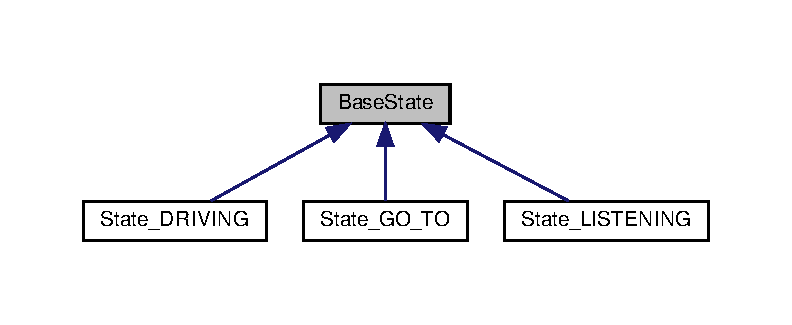
\includegraphics[width=350pt]{class_base_state__inherit__graph}
\end{center}
\end{figure}
\subsection*{Public Member Functions}
\begin{DoxyCompactItemize}
\item 
virtual void \hyperlink{class_base_state_a398bc67a0353c3e8da1597dbdbbba2cc}{drive} (\hyperlink{class_state_machine}{State\+Machine} $\ast$m)=0
\item 
virtual void \hyperlink{class_base_state_ac65db46601f60cd025ff058dae117d7c}{listen} (\hyperlink{class_state_machine}{State\+Machine} $\ast$m)=0
\item 
virtual void \hyperlink{class_base_state_a6acb02c9d6b3e54602e163dc1848ac3a}{go\+\_\+to} (\hyperlink{class_state_machine}{State\+Machine} $\ast$m, string target)=0
\item 
virtual void \hyperlink{class_base_state_a9b21ace3d89308945fdecd81b34d3919}{label} (\hyperlink{class_state_machine}{State\+Machine} $\ast$m, string label)=0
\item 
virtual void \hyperlink{class_base_state_aafa71e762d651f1f5a1f7a6decd0d3b5}{goal\+\_\+reached} (\hyperlink{class_state_machine}{State\+Machine} $\ast$m)=0
\end{DoxyCompactItemize}


\subsection{Detailed Description}
Base class for all the specific state classes. Contains public interface of all derived classes. 

Definition at line 12 of file Base\+State.\+h.



\subsection{Member Function Documentation}
\mbox{\Hypertarget{class_base_state_a398bc67a0353c3e8da1597dbdbbba2cc}\label{class_base_state_a398bc67a0353c3e8da1597dbdbbba2cc}} 
\index{Base\+State@{Base\+State}!drive@{drive}}
\index{drive@{drive}!Base\+State@{Base\+State}}
\subsubsection{\texorpdfstring{drive()}{drive()}}
{\footnotesize\ttfamily virtual void Base\+State\+::drive (\begin{DoxyParamCaption}\item[{\hyperlink{class_state_machine}{State\+Machine} $\ast$}]{m }\end{DoxyParamCaption})\hspace{0.3cm}{\ttfamily [pure virtual]}}



Implemented in \hyperlink{class_state___g_o___t_o_aac09d9440545af49f32c947054bb9fcf}{State\+\_\+\+G\+O\+\_\+\+TO}, \hyperlink{class_state___d_r_i_v_i_n_g_a7239b366223065ebd5bbbff2330efb0c}{State\+\_\+\+D\+R\+I\+V\+I\+NG}, and \hyperlink{class_state___l_i_s_t_e_n_i_n_g_af77af4f01ff6fde1f64b133c5fa61cb8}{State\+\_\+\+L\+I\+S\+T\+E\+N\+I\+NG}.

\mbox{\Hypertarget{class_base_state_a6acb02c9d6b3e54602e163dc1848ac3a}\label{class_base_state_a6acb02c9d6b3e54602e163dc1848ac3a}} 
\index{Base\+State@{Base\+State}!go\+\_\+to@{go\+\_\+to}}
\index{go\+\_\+to@{go\+\_\+to}!Base\+State@{Base\+State}}
\subsubsection{\texorpdfstring{go\+\_\+to()}{go\_to()}}
{\footnotesize\ttfamily virtual void Base\+State\+::go\+\_\+to (\begin{DoxyParamCaption}\item[{\hyperlink{class_state_machine}{State\+Machine} $\ast$}]{m,  }\item[{string}]{target }\end{DoxyParamCaption})\hspace{0.3cm}{\ttfamily [pure virtual]}}



Implemented in \hyperlink{class_state___g_o___t_o_a31cad500afd9332090862e4eac34509a}{State\+\_\+\+G\+O\+\_\+\+TO}, \hyperlink{class_state___d_r_i_v_i_n_g_a83631cdbe860c6fa1b965fe01337bb5f}{State\+\_\+\+D\+R\+I\+V\+I\+NG}, and \hyperlink{class_state___l_i_s_t_e_n_i_n_g_ab6eba322cb293ec2b693f48260f72751}{State\+\_\+\+L\+I\+S\+T\+E\+N\+I\+NG}.

\mbox{\Hypertarget{class_base_state_aafa71e762d651f1f5a1f7a6decd0d3b5}\label{class_base_state_aafa71e762d651f1f5a1f7a6decd0d3b5}} 
\index{Base\+State@{Base\+State}!goal\+\_\+reached@{goal\+\_\+reached}}
\index{goal\+\_\+reached@{goal\+\_\+reached}!Base\+State@{Base\+State}}
\subsubsection{\texorpdfstring{goal\+\_\+reached()}{goal\_reached()}}
{\footnotesize\ttfamily virtual void Base\+State\+::goal\+\_\+reached (\begin{DoxyParamCaption}\item[{\hyperlink{class_state_machine}{State\+Machine} $\ast$}]{m }\end{DoxyParamCaption})\hspace{0.3cm}{\ttfamily [pure virtual]}}



Implemented in \hyperlink{class_state___g_o___t_o_aefada4399e8bfdc2794a7bd4c3fdc065}{State\+\_\+\+G\+O\+\_\+\+TO}, \hyperlink{class_state___d_r_i_v_i_n_g_a73ffdf6352e4cc70ff26a28266497c13}{State\+\_\+\+D\+R\+I\+V\+I\+NG}, and \hyperlink{class_state___l_i_s_t_e_n_i_n_g_a673b6c2cd73588f9db6b252c5e0d6d60}{State\+\_\+\+L\+I\+S\+T\+E\+N\+I\+NG}.

\mbox{\Hypertarget{class_base_state_a9b21ace3d89308945fdecd81b34d3919}\label{class_base_state_a9b21ace3d89308945fdecd81b34d3919}} 
\index{Base\+State@{Base\+State}!label@{label}}
\index{label@{label}!Base\+State@{Base\+State}}
\subsubsection{\texorpdfstring{label()}{label()}}
{\footnotesize\ttfamily virtual void Base\+State\+::label (\begin{DoxyParamCaption}\item[{\hyperlink{class_state_machine}{State\+Machine} $\ast$}]{m,  }\item[{string}]{label }\end{DoxyParamCaption})\hspace{0.3cm}{\ttfamily [pure virtual]}}



Implemented in \hyperlink{class_state___g_o___t_o_a069ecbdf4f8e48e697cebd14da6be795}{State\+\_\+\+G\+O\+\_\+\+TO}, \hyperlink{class_state___d_r_i_v_i_n_g_a3826ccfb3b2b4a63c2f9bc243ea403c8}{State\+\_\+\+D\+R\+I\+V\+I\+NG}, and \hyperlink{class_state___l_i_s_t_e_n_i_n_g_a780b6f499710282279e60c7e48cd6611}{State\+\_\+\+L\+I\+S\+T\+E\+N\+I\+NG}.

\mbox{\Hypertarget{class_base_state_ac65db46601f60cd025ff058dae117d7c}\label{class_base_state_ac65db46601f60cd025ff058dae117d7c}} 
\index{Base\+State@{Base\+State}!listen@{listen}}
\index{listen@{listen}!Base\+State@{Base\+State}}
\subsubsection{\texorpdfstring{listen()}{listen()}}
{\footnotesize\ttfamily virtual void Base\+State\+::listen (\begin{DoxyParamCaption}\item[{\hyperlink{class_state_machine}{State\+Machine} $\ast$}]{m }\end{DoxyParamCaption})\hspace{0.3cm}{\ttfamily [pure virtual]}}



Implemented in \hyperlink{class_state___g_o___t_o_a9ef62ef0417ecbadae9ba02cac1903bd}{State\+\_\+\+G\+O\+\_\+\+TO}, \hyperlink{class_state___d_r_i_v_i_n_g_a35fd6129ede7020827f4a2a8632b1527}{State\+\_\+\+D\+R\+I\+V\+I\+NG}, and \hyperlink{class_state___l_i_s_t_e_n_i_n_g_a0063dbc4d0cc0712e4a69e67a452f92b}{State\+\_\+\+L\+I\+S\+T\+E\+N\+I\+NG}.



The documentation for this class was generated from the following file\+:\begin{DoxyCompactItemize}
\item 
catkin\+\_\+ws/src/labeled\+\_\+slam/include/labeled\+\_\+slam/\+State\+Machine/\hyperlink{_base_state_8h}{Base\+State.\+h}\end{DoxyCompactItemize}

\hypertarget{classcommand__recognition_1_1_main___speech___controller}{}\section{command\+\_\+recognition.\+Main\+\_\+\+Speech\+\_\+\+Controller Class Reference}
\label{classcommand__recognition_1_1_main___speech___controller}\index{command\+\_\+recognition.\+Main\+\_\+\+Speech\+\_\+\+Controller@{command\+\_\+recognition.\+Main\+\_\+\+Speech\+\_\+\+Controller}}


Mother class.  


\subsection*{Public Member Functions}
\begin{DoxyCompactItemize}
\item 
def \hyperlink{classcommand__recognition_1_1_main___speech___controller_abfc55f738b24720625190c078d5de151}{\+\_\+\+\_\+init\+\_\+\+\_\+} (self)
\begin{DoxyCompactList}\small\item\em Initialize global variables like topics and recognizer. \end{DoxyCompactList}\item 
def \hyperlink{classcommand__recognition_1_1_main___speech___controller_a5d05c0bcca81f6fdcea9de648f114291}{recognize\+\_\+speech} (self, \hyperlink{classcommand__recognition_1_1_main___speech___controller_abbf94dd60a0a5244906d8842734eca55}{speech})
\begin{DoxyCompactList}\small\item\em Get the audio signal from the microphone as a string. \end{DoxyCompactList}\item 
def \hyperlink{classcommand__recognition_1_1_main___speech___controller_a8430ad5000f73886dbc9cde072f0d4ba}{recognize\+\_\+command} (self, \hyperlink{classcommand__recognition_1_1_main___speech___controller_abbf94dd60a0a5244906d8842734eca55}{speech}, \hyperlink{classcommand__recognition_1_1_main___speech___controller_a382d3bbe539ba93713ad9b4057e2a226}{speechcommand}, \hyperlink{classcommand__recognition_1_1_main___speech___controller_ace8e299f41b4b37fe5e3e060fa03781f}{mytopic})
\begin{DoxyCompactList}\small\item\em From the audio signal received, publish the desired command. \end{DoxyCompactList}\item 
def \hyperlink{classcommand__recognition_1_1_main___speech___controller_a7b0164a1ceb1c3de76242c77c3b762d5}{recognize\+\_\+user} (self, \hyperlink{classcommand__recognition_1_1_main___speech___controller_abbf94dd60a0a5244906d8842734eca55}{speech}, \hyperlink{classcommand__recognition_1_1_main___speech___controller_a8db8cf2f5d84e14336e83ce65fc79584}{confirmation})
\begin{DoxyCompactList}\small\item\em Ask user for feedback of the recognized speech. \end{DoxyCompactList}\item 
def \hyperlink{classcommand__recognition_1_1_main___speech___controller_a502341d8112e260fc5912eba6620d788}{start\+\_\+recognition} (self)
\begin{DoxyCompactList}\small\item\em The \textquotesingle{}main\textquotesingle{} function of the class, it calls constantly the other. \end{DoxyCompactList}\end{DoxyCompactItemize}
\subsection*{Public Attributes}
\begin{DoxyCompactItemize}
\item 
\hyperlink{classcommand__recognition_1_1_main___speech___controller_ace8e299f41b4b37fe5e3e060fa03781f}{mytopic}
\item 
\hyperlink{classcommand__recognition_1_1_main___speech___controller_abbf94dd60a0a5244906d8842734eca55}{speech}
\item 
\hyperlink{classcommand__recognition_1_1_main___speech___controller_a8db8cf2f5d84e14336e83ce65fc79584}{confirmation}
\item 
\hyperlink{classcommand__recognition_1_1_main___speech___controller_a7b8c9320db0e9e052e46d7261914aa1f}{status}
\item 
\hyperlink{classcommand__recognition_1_1_main___speech___controller_a382d3bbe539ba93713ad9b4057e2a226}{speechcommand}
\end{DoxyCompactItemize}


\subsection{Detailed Description}
Mother class. 

Definition at line 22 of file command\+\_\+recognition.\+py.



\subsection{Constructor \& Destructor Documentation}
\mbox{\Hypertarget{classcommand__recognition_1_1_main___speech___controller_abfc55f738b24720625190c078d5de151}\label{classcommand__recognition_1_1_main___speech___controller_abfc55f738b24720625190c078d5de151}} 
\index{command\+\_\+recognition\+::\+Main\+\_\+\+Speech\+\_\+\+Controller@{command\+\_\+recognition\+::\+Main\+\_\+\+Speech\+\_\+\+Controller}!\+\_\+\+\_\+init\+\_\+\+\_\+@{\+\_\+\+\_\+init\+\_\+\+\_\+}}
\index{\+\_\+\+\_\+init\+\_\+\+\_\+@{\+\_\+\+\_\+init\+\_\+\+\_\+}!command\+\_\+recognition\+::\+Main\+\_\+\+Speech\+\_\+\+Controller@{command\+\_\+recognition\+::\+Main\+\_\+\+Speech\+\_\+\+Controller}}
\subsubsection{\texorpdfstring{\+\_\+\+\_\+init\+\_\+\+\_\+()}{\_\_init\_\_()}}
{\footnotesize\ttfamily def command\+\_\+recognition.\+Main\+\_\+\+Speech\+\_\+\+Controller.\+\_\+\+\_\+init\+\_\+\+\_\+ (\begin{DoxyParamCaption}\item[{}]{self }\end{DoxyParamCaption})}



Initialize global variables like topics and recognizer. 



Definition at line 25 of file command\+\_\+recognition.\+py.



\subsection{Member Function Documentation}
\mbox{\Hypertarget{classcommand__recognition_1_1_main___speech___controller_a8430ad5000f73886dbc9cde072f0d4ba}\label{classcommand__recognition_1_1_main___speech___controller_a8430ad5000f73886dbc9cde072f0d4ba}} 
\index{command\+\_\+recognition\+::\+Main\+\_\+\+Speech\+\_\+\+Controller@{command\+\_\+recognition\+::\+Main\+\_\+\+Speech\+\_\+\+Controller}!recognize\+\_\+command@{recognize\+\_\+command}}
\index{recognize\+\_\+command@{recognize\+\_\+command}!command\+\_\+recognition\+::\+Main\+\_\+\+Speech\+\_\+\+Controller@{command\+\_\+recognition\+::\+Main\+\_\+\+Speech\+\_\+\+Controller}}
\subsubsection{\texorpdfstring{recognize\+\_\+command()}{recognize\_command()}}
{\footnotesize\ttfamily def command\+\_\+recognition.\+Main\+\_\+\+Speech\+\_\+\+Controller.\+recognize\+\_\+command (\begin{DoxyParamCaption}\item[{}]{self,  }\item[{}]{speech,  }\item[{}]{speechcommand,  }\item[{}]{mytopic }\end{DoxyParamCaption})}



From the audio signal received, publish the desired command. 



Definition at line 72 of file command\+\_\+recognition.\+py.

\mbox{\Hypertarget{classcommand__recognition_1_1_main___speech___controller_a5d05c0bcca81f6fdcea9de648f114291}\label{classcommand__recognition_1_1_main___speech___controller_a5d05c0bcca81f6fdcea9de648f114291}} 
\index{command\+\_\+recognition\+::\+Main\+\_\+\+Speech\+\_\+\+Controller@{command\+\_\+recognition\+::\+Main\+\_\+\+Speech\+\_\+\+Controller}!recognize\+\_\+speech@{recognize\+\_\+speech}}
\index{recognize\+\_\+speech@{recognize\+\_\+speech}!command\+\_\+recognition\+::\+Main\+\_\+\+Speech\+\_\+\+Controller@{command\+\_\+recognition\+::\+Main\+\_\+\+Speech\+\_\+\+Controller}}
\subsubsection{\texorpdfstring{recognize\+\_\+speech()}{recognize\_speech()}}
{\footnotesize\ttfamily def command\+\_\+recognition.\+Main\+\_\+\+Speech\+\_\+\+Controller.\+recognize\+\_\+speech (\begin{DoxyParamCaption}\item[{}]{self,  }\item[{}]{speech }\end{DoxyParamCaption})}



Get the audio signal from the microphone as a string. 



Definition at line 45 of file command\+\_\+recognition.\+py.

\mbox{\Hypertarget{classcommand__recognition_1_1_main___speech___controller_a7b0164a1ceb1c3de76242c77c3b762d5}\label{classcommand__recognition_1_1_main___speech___controller_a7b0164a1ceb1c3de76242c77c3b762d5}} 
\index{command\+\_\+recognition\+::\+Main\+\_\+\+Speech\+\_\+\+Controller@{command\+\_\+recognition\+::\+Main\+\_\+\+Speech\+\_\+\+Controller}!recognize\+\_\+user@{recognize\+\_\+user}}
\index{recognize\+\_\+user@{recognize\+\_\+user}!command\+\_\+recognition\+::\+Main\+\_\+\+Speech\+\_\+\+Controller@{command\+\_\+recognition\+::\+Main\+\_\+\+Speech\+\_\+\+Controller}}
\subsubsection{\texorpdfstring{recognize\+\_\+user()}{recognize\_user()}}
{\footnotesize\ttfamily def command\+\_\+recognition.\+Main\+\_\+\+Speech\+\_\+\+Controller.\+recognize\+\_\+user (\begin{DoxyParamCaption}\item[{}]{self,  }\item[{}]{speech,  }\item[{}]{confirmation }\end{DoxyParamCaption})}



Ask user for feedback of the recognized speech. 



Definition at line 168 of file command\+\_\+recognition.\+py.

\mbox{\Hypertarget{classcommand__recognition_1_1_main___speech___controller_a502341d8112e260fc5912eba6620d788}\label{classcommand__recognition_1_1_main___speech___controller_a502341d8112e260fc5912eba6620d788}} 
\index{command\+\_\+recognition\+::\+Main\+\_\+\+Speech\+\_\+\+Controller@{command\+\_\+recognition\+::\+Main\+\_\+\+Speech\+\_\+\+Controller}!start\+\_\+recognition@{start\+\_\+recognition}}
\index{start\+\_\+recognition@{start\+\_\+recognition}!command\+\_\+recognition\+::\+Main\+\_\+\+Speech\+\_\+\+Controller@{command\+\_\+recognition\+::\+Main\+\_\+\+Speech\+\_\+\+Controller}}
\subsubsection{\texorpdfstring{start\+\_\+recognition()}{start\_recognition()}}
{\footnotesize\ttfamily def command\+\_\+recognition.\+Main\+\_\+\+Speech\+\_\+\+Controller.\+start\+\_\+recognition (\begin{DoxyParamCaption}\item[{}]{self }\end{DoxyParamCaption})}



The \textquotesingle{}main\textquotesingle{} function of the class, it calls constantly the other. 



Definition at line 190 of file command\+\_\+recognition.\+py.



\subsection{Member Data Documentation}
\mbox{\Hypertarget{classcommand__recognition_1_1_main___speech___controller_a8db8cf2f5d84e14336e83ce65fc79584}\label{classcommand__recognition_1_1_main___speech___controller_a8db8cf2f5d84e14336e83ce65fc79584}} 
\index{command\+\_\+recognition\+::\+Main\+\_\+\+Speech\+\_\+\+Controller@{command\+\_\+recognition\+::\+Main\+\_\+\+Speech\+\_\+\+Controller}!confirmation@{confirmation}}
\index{confirmation@{confirmation}!command\+\_\+recognition\+::\+Main\+\_\+\+Speech\+\_\+\+Controller@{command\+\_\+recognition\+::\+Main\+\_\+\+Speech\+\_\+\+Controller}}
\subsubsection{\texorpdfstring{confirmation}{confirmation}}
{\footnotesize\ttfamily command\+\_\+recognition.\+Main\+\_\+\+Speech\+\_\+\+Controller.\+confirmation}



Definition at line 34 of file command\+\_\+recognition.\+py.

\mbox{\Hypertarget{classcommand__recognition_1_1_main___speech___controller_ace8e299f41b4b37fe5e3e060fa03781f}\label{classcommand__recognition_1_1_main___speech___controller_ace8e299f41b4b37fe5e3e060fa03781f}} 
\index{command\+\_\+recognition\+::\+Main\+\_\+\+Speech\+\_\+\+Controller@{command\+\_\+recognition\+::\+Main\+\_\+\+Speech\+\_\+\+Controller}!mytopic@{mytopic}}
\index{mytopic@{mytopic}!command\+\_\+recognition\+::\+Main\+\_\+\+Speech\+\_\+\+Controller@{command\+\_\+recognition\+::\+Main\+\_\+\+Speech\+\_\+\+Controller}}
\subsubsection{\texorpdfstring{mytopic}{mytopic}}
{\footnotesize\ttfamily command\+\_\+recognition.\+Main\+\_\+\+Speech\+\_\+\+Controller.\+mytopic}



Definition at line 28 of file command\+\_\+recognition.\+py.

\mbox{\Hypertarget{classcommand__recognition_1_1_main___speech___controller_abbf94dd60a0a5244906d8842734eca55}\label{classcommand__recognition_1_1_main___speech___controller_abbf94dd60a0a5244906d8842734eca55}} 
\index{command\+\_\+recognition\+::\+Main\+\_\+\+Speech\+\_\+\+Controller@{command\+\_\+recognition\+::\+Main\+\_\+\+Speech\+\_\+\+Controller}!speech@{speech}}
\index{speech@{speech}!command\+\_\+recognition\+::\+Main\+\_\+\+Speech\+\_\+\+Controller@{command\+\_\+recognition\+::\+Main\+\_\+\+Speech\+\_\+\+Controller}}
\subsubsection{\texorpdfstring{speech}{speech}}
{\footnotesize\ttfamily command\+\_\+recognition.\+Main\+\_\+\+Speech\+\_\+\+Controller.\+speech}



Definition at line 31 of file command\+\_\+recognition.\+py.

\mbox{\Hypertarget{classcommand__recognition_1_1_main___speech___controller_a382d3bbe539ba93713ad9b4057e2a226}\label{classcommand__recognition_1_1_main___speech___controller_a382d3bbe539ba93713ad9b4057e2a226}} 
\index{command\+\_\+recognition\+::\+Main\+\_\+\+Speech\+\_\+\+Controller@{command\+\_\+recognition\+::\+Main\+\_\+\+Speech\+\_\+\+Controller}!speechcommand@{speechcommand}}
\index{speechcommand@{speechcommand}!command\+\_\+recognition\+::\+Main\+\_\+\+Speech\+\_\+\+Controller@{command\+\_\+recognition\+::\+Main\+\_\+\+Speech\+\_\+\+Controller}}
\subsubsection{\texorpdfstring{speechcommand}{speechcommand}}
{\footnotesize\ttfamily command\+\_\+recognition.\+Main\+\_\+\+Speech\+\_\+\+Controller.\+speechcommand}



Definition at line 40 of file command\+\_\+recognition.\+py.

\mbox{\Hypertarget{classcommand__recognition_1_1_main___speech___controller_a7b8c9320db0e9e052e46d7261914aa1f}\label{classcommand__recognition_1_1_main___speech___controller_a7b8c9320db0e9e052e46d7261914aa1f}} 
\index{command\+\_\+recognition\+::\+Main\+\_\+\+Speech\+\_\+\+Controller@{command\+\_\+recognition\+::\+Main\+\_\+\+Speech\+\_\+\+Controller}!status@{status}}
\index{status@{status}!command\+\_\+recognition\+::\+Main\+\_\+\+Speech\+\_\+\+Controller@{command\+\_\+recognition\+::\+Main\+\_\+\+Speech\+\_\+\+Controller}}
\subsubsection{\texorpdfstring{status}{status}}
{\footnotesize\ttfamily command\+\_\+recognition.\+Main\+\_\+\+Speech\+\_\+\+Controller.\+status}



Definition at line 37 of file command\+\_\+recognition.\+py.



The documentation for this class was generated from the following file\+:\begin{DoxyCompactItemize}
\item 
catkin\+\_\+ws/src/labeled\+\_\+slam/src/\hyperlink{command__recognition_8py}{command\+\_\+recognition.\+py}\end{DoxyCompactItemize}

\hypertarget{class_state___d_r_i_v_i_n_g}{}\section{State\+\_\+\+D\+R\+I\+V\+I\+NG Class Reference}
\label{class_state___d_r_i_v_i_n_g}\index{State\+\_\+\+D\+R\+I\+V\+I\+NG@{State\+\_\+\+D\+R\+I\+V\+I\+NG}}


State class for the mode, when the robot is controlled manually using the smartwatch.  




{\ttfamily \#include $<$State\+\_\+\+D\+R\+I\+V\+I\+N\+G.\+h$>$}



Inheritance diagram for State\+\_\+\+D\+R\+I\+V\+I\+NG\+:
\nopagebreak
\begin{figure}[H]
\begin{center}
\leavevmode
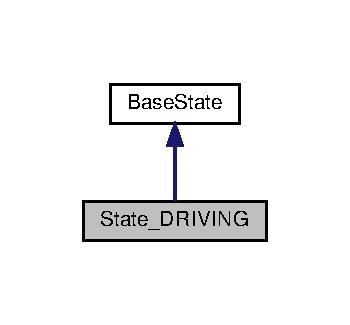
\includegraphics[width=168pt]{class_state___d_r_i_v_i_n_g__inherit__graph}
\end{center}
\end{figure}


Collaboration diagram for State\+\_\+\+D\+R\+I\+V\+I\+NG\+:
\nopagebreak
\begin{figure}[H]
\begin{center}
\leavevmode
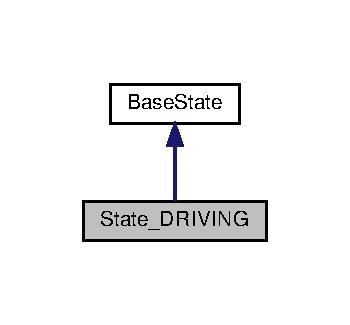
\includegraphics[width=168pt]{class_state___d_r_i_v_i_n_g__coll__graph}
\end{center}
\end{figure}
\subsection*{Public Member Functions}
\begin{DoxyCompactItemize}
\item 
\hyperlink{class_state___d_r_i_v_i_n_g_a54b0c8690994358c52b409d17bc413b5}{State\+\_\+\+D\+R\+I\+V\+I\+NG} (\hyperlink{class_state_machine}{State\+Machine} $\ast$m)
\begin{DoxyCompactList}\small\item\em Constructor of \hyperlink{class_state___d_r_i_v_i_n_g}{State\+\_\+\+D\+R\+I\+V\+I\+NG}. \end{DoxyCompactList}\item 
\hyperlink{class_state___d_r_i_v_i_n_g_a0770c3991f746520e21e1c7e12610f1d}{$\sim$\+State\+\_\+\+D\+R\+I\+V\+I\+NG} ()
\begin{DoxyCompactList}\small\item\em Destructor of \hyperlink{class_state___d_r_i_v_i_n_g}{State\+\_\+\+D\+R\+I\+V\+I\+NG}. \end{DoxyCompactList}\item 
virtual void \hyperlink{class_state___d_r_i_v_i_n_g_a7239b366223065ebd5bbbff2330efb0c}{drive} (\hyperlink{class_state_machine}{State\+Machine} $\ast$m)
\begin{DoxyCompactList}\small\item\em Don\textquotesingle{}t do anythin on command drive. \end{DoxyCompactList}\item 
virtual void \hyperlink{class_state___d_r_i_v_i_n_g_a35fd6129ede7020827f4a2a8632b1527}{listen} (\hyperlink{class_state_machine}{State\+Machine} $\ast$m)
\begin{DoxyCompactList}\small\item\em Switch to listening mode. \end{DoxyCompactList}\item 
virtual void \hyperlink{class_state___d_r_i_v_i_n_g_a83631cdbe860c6fa1b965fe01337bb5f}{go\+\_\+to} (\hyperlink{class_state_machine}{State\+Machine} $\ast$m, string target)
\begin{DoxyCompactList}\small\item\em Don\textquotesingle{}t do anythin on command go\+\_\+to. \end{DoxyCompactList}\item 
virtual void \hyperlink{class_state___d_r_i_v_i_n_g_a3826ccfb3b2b4a63c2f9bc243ea403c8}{label} (\hyperlink{class_state_machine}{State\+Machine} $\ast$m, string label)
\begin{DoxyCompactList}\small\item\em Don\textquotesingle{}t do anything on command label. \end{DoxyCompactList}\item 
virtual void \hyperlink{class_state___d_r_i_v_i_n_g_a73ffdf6352e4cc70ff26a28266497c13}{goal\+\_\+reached} (\hyperlink{class_state_machine}{State\+Machine} $\ast$m)
\begin{DoxyCompactList}\small\item\em Don\textquotesingle{}t do anything when goal reached is received. \end{DoxyCompactList}\end{DoxyCompactItemize}


\subsection{Detailed Description}
State class for the mode, when the robot is controlled manually using the smartwatch. 

Definition at line 10 of file State\+\_\+\+D\+R\+I\+V\+I\+N\+G.\+h.



\subsection{Constructor \& Destructor Documentation}
\mbox{\Hypertarget{class_state___d_r_i_v_i_n_g_a54b0c8690994358c52b409d17bc413b5}\label{class_state___d_r_i_v_i_n_g_a54b0c8690994358c52b409d17bc413b5}} 
\index{State\+\_\+\+D\+R\+I\+V\+I\+NG@{State\+\_\+\+D\+R\+I\+V\+I\+NG}!State\+\_\+\+D\+R\+I\+V\+I\+NG@{State\+\_\+\+D\+R\+I\+V\+I\+NG}}
\index{State\+\_\+\+D\+R\+I\+V\+I\+NG@{State\+\_\+\+D\+R\+I\+V\+I\+NG}!State\+\_\+\+D\+R\+I\+V\+I\+NG@{State\+\_\+\+D\+R\+I\+V\+I\+NG}}
\subsubsection{\texorpdfstring{State\+\_\+\+D\+R\+I\+V\+I\+N\+G()}{State\_DRIVING()}}
{\footnotesize\ttfamily State\+\_\+\+D\+R\+I\+V\+I\+N\+G\+::\+State\+\_\+\+D\+R\+I\+V\+I\+NG (\begin{DoxyParamCaption}\item[{\hyperlink{class_state_machine}{State\+Machine} $\ast$}]{m }\end{DoxyParamCaption})}



Constructor of \hyperlink{class_state___d_r_i_v_i_n_g}{State\+\_\+\+D\+R\+I\+V\+I\+NG}. 

Calls service activate\+\_\+driving (always, when this state is entered) with a T\+R\+UE flag 

Definition at line 11 of file State\+\_\+\+D\+R\+I\+V\+I\+N\+G.\+cpp.

\mbox{\Hypertarget{class_state___d_r_i_v_i_n_g_a0770c3991f746520e21e1c7e12610f1d}\label{class_state___d_r_i_v_i_n_g_a0770c3991f746520e21e1c7e12610f1d}} 
\index{State\+\_\+\+D\+R\+I\+V\+I\+NG@{State\+\_\+\+D\+R\+I\+V\+I\+NG}!````~State\+\_\+\+D\+R\+I\+V\+I\+NG@{$\sim$\+State\+\_\+\+D\+R\+I\+V\+I\+NG}}
\index{````~State\+\_\+\+D\+R\+I\+V\+I\+NG@{$\sim$\+State\+\_\+\+D\+R\+I\+V\+I\+NG}!State\+\_\+\+D\+R\+I\+V\+I\+NG@{State\+\_\+\+D\+R\+I\+V\+I\+NG}}
\subsubsection{\texorpdfstring{$\sim$\+State\+\_\+\+D\+R\+I\+V\+I\+N\+G()}{~State\_DRIVING()}}
{\footnotesize\ttfamily State\+\_\+\+D\+R\+I\+V\+I\+N\+G\+::$\sim$\+State\+\_\+\+D\+R\+I\+V\+I\+NG (\begin{DoxyParamCaption}{ }\end{DoxyParamCaption})}



Destructor of \hyperlink{class_state___d_r_i_v_i_n_g}{State\+\_\+\+D\+R\+I\+V\+I\+NG}. 

Calls service activate\+\_\+driving (always, when this state is left) with a F\+A\+L\+SE flag 

Definition at line 30 of file State\+\_\+\+D\+R\+I\+V\+I\+N\+G.\+cpp.



\subsection{Member Function Documentation}
\mbox{\Hypertarget{class_state___d_r_i_v_i_n_g_a7239b366223065ebd5bbbff2330efb0c}\label{class_state___d_r_i_v_i_n_g_a7239b366223065ebd5bbbff2330efb0c}} 
\index{State\+\_\+\+D\+R\+I\+V\+I\+NG@{State\+\_\+\+D\+R\+I\+V\+I\+NG}!drive@{drive}}
\index{drive@{drive}!State\+\_\+\+D\+R\+I\+V\+I\+NG@{State\+\_\+\+D\+R\+I\+V\+I\+NG}}
\subsubsection{\texorpdfstring{drive()}{drive()}}
{\footnotesize\ttfamily void State\+\_\+\+D\+R\+I\+V\+I\+N\+G\+::drive (\begin{DoxyParamCaption}\item[{\hyperlink{class_state_machine}{State\+Machine} $\ast$}]{m }\end{DoxyParamCaption})\hspace{0.3cm}{\ttfamily [virtual]}}



Don\textquotesingle{}t do anythin on command drive. 



Implements \hyperlink{class_base_state_a398bc67a0353c3e8da1597dbdbbba2cc}{Base\+State}.



Definition at line 45 of file State\+\_\+\+D\+R\+I\+V\+I\+N\+G.\+cpp.

\mbox{\Hypertarget{class_state___d_r_i_v_i_n_g_a83631cdbe860c6fa1b965fe01337bb5f}\label{class_state___d_r_i_v_i_n_g_a83631cdbe860c6fa1b965fe01337bb5f}} 
\index{State\+\_\+\+D\+R\+I\+V\+I\+NG@{State\+\_\+\+D\+R\+I\+V\+I\+NG}!go\+\_\+to@{go\+\_\+to}}
\index{go\+\_\+to@{go\+\_\+to}!State\+\_\+\+D\+R\+I\+V\+I\+NG@{State\+\_\+\+D\+R\+I\+V\+I\+NG}}
\subsubsection{\texorpdfstring{go\+\_\+to()}{go\_to()}}
{\footnotesize\ttfamily void State\+\_\+\+D\+R\+I\+V\+I\+N\+G\+::go\+\_\+to (\begin{DoxyParamCaption}\item[{\hyperlink{class_state_machine}{State\+Machine} $\ast$}]{m,  }\item[{string}]{target }\end{DoxyParamCaption})\hspace{0.3cm}{\ttfamily [virtual]}}



Don\textquotesingle{}t do anythin on command go\+\_\+to. 



Implements \hyperlink{class_base_state_a6acb02c9d6b3e54602e163dc1848ac3a}{Base\+State}.



Definition at line 63 of file State\+\_\+\+D\+R\+I\+V\+I\+N\+G.\+cpp.

\mbox{\Hypertarget{class_state___d_r_i_v_i_n_g_a73ffdf6352e4cc70ff26a28266497c13}\label{class_state___d_r_i_v_i_n_g_a73ffdf6352e4cc70ff26a28266497c13}} 
\index{State\+\_\+\+D\+R\+I\+V\+I\+NG@{State\+\_\+\+D\+R\+I\+V\+I\+NG}!goal\+\_\+reached@{goal\+\_\+reached}}
\index{goal\+\_\+reached@{goal\+\_\+reached}!State\+\_\+\+D\+R\+I\+V\+I\+NG@{State\+\_\+\+D\+R\+I\+V\+I\+NG}}
\subsubsection{\texorpdfstring{goal\+\_\+reached()}{goal\_reached()}}
{\footnotesize\ttfamily void State\+\_\+\+D\+R\+I\+V\+I\+N\+G\+::goal\+\_\+reached (\begin{DoxyParamCaption}\item[{\hyperlink{class_state_machine}{State\+Machine} $\ast$}]{m }\end{DoxyParamCaption})\hspace{0.3cm}{\ttfamily [virtual]}}



Don\textquotesingle{}t do anything when goal reached is received. 



Implements \hyperlink{class_base_state_aafa71e762d651f1f5a1f7a6decd0d3b5}{Base\+State}.



Definition at line 79 of file State\+\_\+\+D\+R\+I\+V\+I\+N\+G.\+cpp.

\mbox{\Hypertarget{class_state___d_r_i_v_i_n_g_a3826ccfb3b2b4a63c2f9bc243ea403c8}\label{class_state___d_r_i_v_i_n_g_a3826ccfb3b2b4a63c2f9bc243ea403c8}} 
\index{State\+\_\+\+D\+R\+I\+V\+I\+NG@{State\+\_\+\+D\+R\+I\+V\+I\+NG}!label@{label}}
\index{label@{label}!State\+\_\+\+D\+R\+I\+V\+I\+NG@{State\+\_\+\+D\+R\+I\+V\+I\+NG}}
\subsubsection{\texorpdfstring{label()}{label()}}
{\footnotesize\ttfamily void State\+\_\+\+D\+R\+I\+V\+I\+N\+G\+::label (\begin{DoxyParamCaption}\item[{\hyperlink{class_state_machine}{State\+Machine} $\ast$}]{m,  }\item[{string}]{label }\end{DoxyParamCaption})\hspace{0.3cm}{\ttfamily [virtual]}}



Don\textquotesingle{}t do anything on command label. 



Implements \hyperlink{class_base_state_a9b21ace3d89308945fdecd81b34d3919}{Base\+State}.



Definition at line 71 of file State\+\_\+\+D\+R\+I\+V\+I\+N\+G.\+cpp.

\mbox{\Hypertarget{class_state___d_r_i_v_i_n_g_a35fd6129ede7020827f4a2a8632b1527}\label{class_state___d_r_i_v_i_n_g_a35fd6129ede7020827f4a2a8632b1527}} 
\index{State\+\_\+\+D\+R\+I\+V\+I\+NG@{State\+\_\+\+D\+R\+I\+V\+I\+NG}!listen@{listen}}
\index{listen@{listen}!State\+\_\+\+D\+R\+I\+V\+I\+NG@{State\+\_\+\+D\+R\+I\+V\+I\+NG}}
\subsubsection{\texorpdfstring{listen()}{listen()}}
{\footnotesize\ttfamily void State\+\_\+\+D\+R\+I\+V\+I\+N\+G\+::listen (\begin{DoxyParamCaption}\item[{\hyperlink{class_state_machine}{State\+Machine} $\ast$}]{m }\end{DoxyParamCaption})\hspace{0.3cm}{\ttfamily [virtual]}}



Switch to listening mode. 



Implements \hyperlink{class_base_state_ac65db46601f60cd025ff058dae117d7c}{Base\+State}.



Definition at line 53 of file State\+\_\+\+D\+R\+I\+V\+I\+N\+G.\+cpp.



The documentation for this class was generated from the following files\+:\begin{DoxyCompactItemize}
\item 
catkin\+\_\+ws/src/labeled\+\_\+slam/include/labeled\+\_\+slam/\+State\+Machine/\hyperlink{_state___d_r_i_v_i_n_g_8h}{State\+\_\+\+D\+R\+I\+V\+I\+N\+G.\+h}\item 
catkin\+\_\+ws/src/labeled\+\_\+slam/src/\+State\+Machine/\hyperlink{_state___d_r_i_v_i_n_g_8cpp}{State\+\_\+\+D\+R\+I\+V\+I\+N\+G.\+cpp}\end{DoxyCompactItemize}

\hypertarget{class_state___g_o___t_o}{}\section{State\+\_\+\+G\+O\+\_\+\+TO Class Reference}
\label{class_state___g_o___t_o}\index{State\+\_\+\+G\+O\+\_\+\+TO@{State\+\_\+\+G\+O\+\_\+\+TO}}


State class for the mode, when the system is following a path towards a target.  




{\ttfamily \#include $<$State\+\_\+\+G\+O\+\_\+\+T\+O.\+h$>$}



Inheritance diagram for State\+\_\+\+G\+O\+\_\+\+TO\+:\nopagebreak
\begin{figure}[H]
\begin{center}
\leavevmode
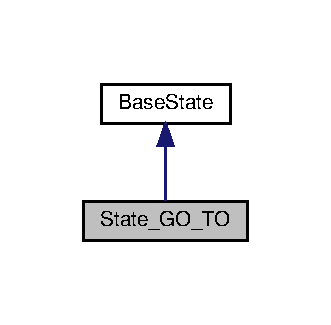
\includegraphics[width=159pt]{class_state___g_o___t_o__inherit__graph}
\end{center}
\end{figure}


Collaboration diagram for State\+\_\+\+G\+O\+\_\+\+TO\+:\nopagebreak
\begin{figure}[H]
\begin{center}
\leavevmode
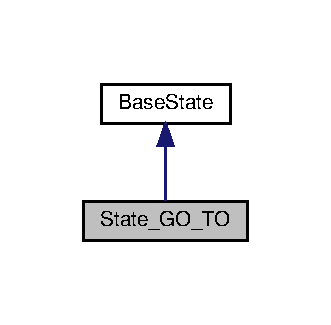
\includegraphics[width=159pt]{class_state___g_o___t_o__coll__graph}
\end{center}
\end{figure}
\subsection*{Public Member Functions}
\begin{DoxyCompactItemize}
\item 
\hyperlink{class_state___g_o___t_o_ad200bcfa107cbd4b1df514f074dcbf2d}{State\+\_\+\+G\+O\+\_\+\+TO} (\hyperlink{class_state_machine}{State\+Machine} $\ast$m, string target)
\begin{DoxyCompactList}\small\item\em Constructor of \hyperlink{class_state___g_o___t_o}{State\+\_\+\+G\+O\+\_\+\+TO}. \end{DoxyCompactList}\item 
\hyperlink{class_state___g_o___t_o_a1f796efa57a876af5d85d1cbe92c48f2}{$\sim$\+State\+\_\+\+G\+O\+\_\+\+TO} ()
\begin{DoxyCompactList}\small\item\em Destructor of \hyperlink{class_state___g_o___t_o}{State\+\_\+\+G\+O\+\_\+\+TO}. \end{DoxyCompactList}\item 
virtual void \hyperlink{class_state___g_o___t_o_aac09d9440545af49f32c947054bb9fcf}{drive} (\hyperlink{class_state_machine}{State\+Machine} $\ast$m)
\begin{DoxyCompactList}\small\item\em Don\textquotesingle{}t do anything on command drive. \end{DoxyCompactList}\item 
virtual void \hyperlink{class_state___g_o___t_o_a9ef62ef0417ecbadae9ba02cac1903bd}{listen} (\hyperlink{class_state_machine}{State\+Machine} $\ast$m)
\begin{DoxyCompactList}\small\item\em Switch to listening mode. \end{DoxyCompactList}\item 
virtual void \hyperlink{class_state___g_o___t_o_a31cad500afd9332090862e4eac34509a}{go\+\_\+to} (\hyperlink{class_state_machine}{State\+Machine} $\ast$m, string target)
\begin{DoxyCompactList}\small\item\em Don\textquotesingle{}t do anything on command go to. \end{DoxyCompactList}\item 
virtual void \hyperlink{class_state___g_o___t_o_a069ecbdf4f8e48e697cebd14da6be795}{label} (\hyperlink{class_state_machine}{State\+Machine} $\ast$m, string label)
\begin{DoxyCompactList}\small\item\em Don\textquotesingle{}t do anything on command label. \end{DoxyCompactList}\item 
virtual void \hyperlink{class_state___g_o___t_o_aefada4399e8bfdc2794a7bd4c3fdc065}{goal\+\_\+reached} (\hyperlink{class_state_machine}{State\+Machine} $\ast$m)
\begin{DoxyCompactList}\small\item\em When goal reached is received, switch back to listening mode (leave this state) \end{DoxyCompactList}\end{DoxyCompactItemize}


\subsection{Detailed Description}
State class for the mode, when the system is following a path towards a target. 

Target can be one of the labels which have been created before 

Definition at line 12 of file State\+\_\+\+G\+O\+\_\+\+T\+O.\+h.



\subsection{Constructor \& Destructor Documentation}
\mbox{\Hypertarget{class_state___g_o___t_o_ad200bcfa107cbd4b1df514f074dcbf2d}\label{class_state___g_o___t_o_ad200bcfa107cbd4b1df514f074dcbf2d}} 
\index{State\+\_\+\+G\+O\+\_\+\+TO@{State\+\_\+\+G\+O\+\_\+\+TO}!State\+\_\+\+G\+O\+\_\+\+TO@{State\+\_\+\+G\+O\+\_\+\+TO}}
\index{State\+\_\+\+G\+O\+\_\+\+TO@{State\+\_\+\+G\+O\+\_\+\+TO}!State\+\_\+\+G\+O\+\_\+\+TO@{State\+\_\+\+G\+O\+\_\+\+TO}}
\subsubsection{\texorpdfstring{State\+\_\+\+G\+O\+\_\+\+T\+O()}{State\_GO\_TO()}}
{\footnotesize\ttfamily State\+\_\+\+G\+O\+\_\+\+T\+O\+::\+State\+\_\+\+G\+O\+\_\+\+TO (\begin{DoxyParamCaption}\item[{\hyperlink{class_state_machine}{State\+Machine} $\ast$}]{m,  }\item[{string}]{target }\end{DoxyParamCaption})}



Constructor of \hyperlink{class_state___g_o___t_o}{State\+\_\+\+G\+O\+\_\+\+TO}. 

Always, when this state is entered\+: (1) Calls service activate\+\_\+path\+\_\+following with a T\+R\+UE flag (2) Calls service which sets the goal to the rtabmap 

Definition at line 13 of file State\+\_\+\+G\+O\+\_\+\+T\+O.\+cpp.

\mbox{\Hypertarget{class_state___g_o___t_o_a1f796efa57a876af5d85d1cbe92c48f2}\label{class_state___g_o___t_o_a1f796efa57a876af5d85d1cbe92c48f2}} 
\index{State\+\_\+\+G\+O\+\_\+\+TO@{State\+\_\+\+G\+O\+\_\+\+TO}!````~State\+\_\+\+G\+O\+\_\+\+TO@{$\sim$\+State\+\_\+\+G\+O\+\_\+\+TO}}
\index{````~State\+\_\+\+G\+O\+\_\+\+TO@{$\sim$\+State\+\_\+\+G\+O\+\_\+\+TO}!State\+\_\+\+G\+O\+\_\+\+TO@{State\+\_\+\+G\+O\+\_\+\+TO}}
\subsubsection{\texorpdfstring{$\sim$\+State\+\_\+\+G\+O\+\_\+\+T\+O()}{~State\_GO\_TO()}}
{\footnotesize\ttfamily State\+\_\+\+G\+O\+\_\+\+T\+O\+::$\sim$\+State\+\_\+\+G\+O\+\_\+\+TO (\begin{DoxyParamCaption}{ }\end{DoxyParamCaption})}



Destructor of \hyperlink{class_state___g_o___t_o}{State\+\_\+\+G\+O\+\_\+\+TO}. 

Calls service activate\+\_\+path\+\_\+following (always, when this state is left) with a F\+A\+L\+SE flag 

Definition at line 45 of file State\+\_\+\+G\+O\+\_\+\+T\+O.\+cpp.



\subsection{Member Function Documentation}
\mbox{\Hypertarget{class_state___g_o___t_o_aac09d9440545af49f32c947054bb9fcf}\label{class_state___g_o___t_o_aac09d9440545af49f32c947054bb9fcf}} 
\index{State\+\_\+\+G\+O\+\_\+\+TO@{State\+\_\+\+G\+O\+\_\+\+TO}!drive@{drive}}
\index{drive@{drive}!State\+\_\+\+G\+O\+\_\+\+TO@{State\+\_\+\+G\+O\+\_\+\+TO}}
\subsubsection{\texorpdfstring{drive()}{drive()}}
{\footnotesize\ttfamily void State\+\_\+\+G\+O\+\_\+\+T\+O\+::drive (\begin{DoxyParamCaption}\item[{\hyperlink{class_state_machine}{State\+Machine} $\ast$}]{m }\end{DoxyParamCaption})\hspace{0.3cm}{\ttfamily [virtual]}}



Don\textquotesingle{}t do anything on command drive. 



Implements \hyperlink{class_base_state_a398bc67a0353c3e8da1597dbdbbba2cc}{Base\+State}.



Definition at line 61 of file State\+\_\+\+G\+O\+\_\+\+T\+O.\+cpp.

\mbox{\Hypertarget{class_state___g_o___t_o_a31cad500afd9332090862e4eac34509a}\label{class_state___g_o___t_o_a31cad500afd9332090862e4eac34509a}} 
\index{State\+\_\+\+G\+O\+\_\+\+TO@{State\+\_\+\+G\+O\+\_\+\+TO}!go\+\_\+to@{go\+\_\+to}}
\index{go\+\_\+to@{go\+\_\+to}!State\+\_\+\+G\+O\+\_\+\+TO@{State\+\_\+\+G\+O\+\_\+\+TO}}
\subsubsection{\texorpdfstring{go\+\_\+to()}{go\_to()}}
{\footnotesize\ttfamily void State\+\_\+\+G\+O\+\_\+\+T\+O\+::go\+\_\+to (\begin{DoxyParamCaption}\item[{\hyperlink{class_state_machine}{State\+Machine} $\ast$}]{m,  }\item[{string}]{target }\end{DoxyParamCaption})\hspace{0.3cm}{\ttfamily [virtual]}}



Don\textquotesingle{}t do anything on command go to. 



Implements \hyperlink{class_base_state_a6acb02c9d6b3e54602e163dc1848ac3a}{Base\+State}.



Definition at line 79 of file State\+\_\+\+G\+O\+\_\+\+T\+O.\+cpp.

\mbox{\Hypertarget{class_state___g_o___t_o_aefada4399e8bfdc2794a7bd4c3fdc065}\label{class_state___g_o___t_o_aefada4399e8bfdc2794a7bd4c3fdc065}} 
\index{State\+\_\+\+G\+O\+\_\+\+TO@{State\+\_\+\+G\+O\+\_\+\+TO}!goal\+\_\+reached@{goal\+\_\+reached}}
\index{goal\+\_\+reached@{goal\+\_\+reached}!State\+\_\+\+G\+O\+\_\+\+TO@{State\+\_\+\+G\+O\+\_\+\+TO}}
\subsubsection{\texorpdfstring{goal\+\_\+reached()}{goal\_reached()}}
{\footnotesize\ttfamily void State\+\_\+\+G\+O\+\_\+\+T\+O\+::goal\+\_\+reached (\begin{DoxyParamCaption}\item[{\hyperlink{class_state_machine}{State\+Machine} $\ast$}]{m }\end{DoxyParamCaption})\hspace{0.3cm}{\ttfamily [virtual]}}



When goal reached is received, switch back to listening mode (leave this state) 



Implements \hyperlink{class_base_state_aafa71e762d651f1f5a1f7a6decd0d3b5}{Base\+State}.



Definition at line 95 of file State\+\_\+\+G\+O\+\_\+\+T\+O.\+cpp.

\mbox{\Hypertarget{class_state___g_o___t_o_a069ecbdf4f8e48e697cebd14da6be795}\label{class_state___g_o___t_o_a069ecbdf4f8e48e697cebd14da6be795}} 
\index{State\+\_\+\+G\+O\+\_\+\+TO@{State\+\_\+\+G\+O\+\_\+\+TO}!label@{label}}
\index{label@{label}!State\+\_\+\+G\+O\+\_\+\+TO@{State\+\_\+\+G\+O\+\_\+\+TO}}
\subsubsection{\texorpdfstring{label()}{label()}}
{\footnotesize\ttfamily void State\+\_\+\+G\+O\+\_\+\+T\+O\+::label (\begin{DoxyParamCaption}\item[{\hyperlink{class_state_machine}{State\+Machine} $\ast$}]{m,  }\item[{string}]{label }\end{DoxyParamCaption})\hspace{0.3cm}{\ttfamily [virtual]}}



Don\textquotesingle{}t do anything on command label. 



Implements \hyperlink{class_base_state_a9b21ace3d89308945fdecd81b34d3919}{Base\+State}.



Definition at line 87 of file State\+\_\+\+G\+O\+\_\+\+T\+O.\+cpp.

\mbox{\Hypertarget{class_state___g_o___t_o_a9ef62ef0417ecbadae9ba02cac1903bd}\label{class_state___g_o___t_o_a9ef62ef0417ecbadae9ba02cac1903bd}} 
\index{State\+\_\+\+G\+O\+\_\+\+TO@{State\+\_\+\+G\+O\+\_\+\+TO}!listen@{listen}}
\index{listen@{listen}!State\+\_\+\+G\+O\+\_\+\+TO@{State\+\_\+\+G\+O\+\_\+\+TO}}
\subsubsection{\texorpdfstring{listen()}{listen()}}
{\footnotesize\ttfamily void State\+\_\+\+G\+O\+\_\+\+T\+O\+::listen (\begin{DoxyParamCaption}\item[{\hyperlink{class_state_machine}{State\+Machine} $\ast$}]{m }\end{DoxyParamCaption})\hspace{0.3cm}{\ttfamily [virtual]}}



Switch to listening mode. 



Implements \hyperlink{class_base_state_ac65db46601f60cd025ff058dae117d7c}{Base\+State}.



Definition at line 69 of file State\+\_\+\+G\+O\+\_\+\+T\+O.\+cpp.



The documentation for this class was generated from the following files\+:\begin{DoxyCompactItemize}
\item 
catkin\+\_\+ws/src/labeled\+\_\+slam/include/labeled\+\_\+slam/\+State\+Machine/\hyperlink{_state___g_o___t_o_8h}{State\+\_\+\+G\+O\+\_\+\+T\+O.\+h}\item 
catkin\+\_\+ws/src/labeled\+\_\+slam/src/\+State\+Machine/\hyperlink{_state___g_o___t_o_8cpp}{State\+\_\+\+G\+O\+\_\+\+T\+O.\+cpp}\end{DoxyCompactItemize}

\hypertarget{class_state___l_i_s_t_e_n_i_n_g}{}\section{State\+\_\+\+L\+I\+S\+T\+E\+N\+I\+NG Class Reference}
\label{class_state___l_i_s_t_e_n_i_n_g}\index{State\+\_\+\+L\+I\+S\+T\+E\+N\+I\+NG@{State\+\_\+\+L\+I\+S\+T\+E\+N\+I\+NG}}


State class for the mode, when the system is listening to voice commands.  




{\ttfamily \#include $<$State\+\_\+\+L\+I\+S\+T\+E\+N\+I\+N\+G.\+h$>$}



Inheritance diagram for State\+\_\+\+L\+I\+S\+T\+E\+N\+I\+NG\+:
\nopagebreak
\begin{figure}[H]
\begin{center}
\leavevmode
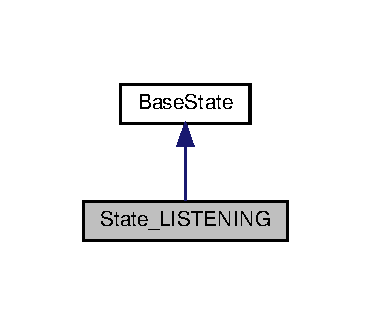
\includegraphics[width=178pt]{class_state___l_i_s_t_e_n_i_n_g__inherit__graph}
\end{center}
\end{figure}


Collaboration diagram for State\+\_\+\+L\+I\+S\+T\+E\+N\+I\+NG\+:
\nopagebreak
\begin{figure}[H]
\begin{center}
\leavevmode
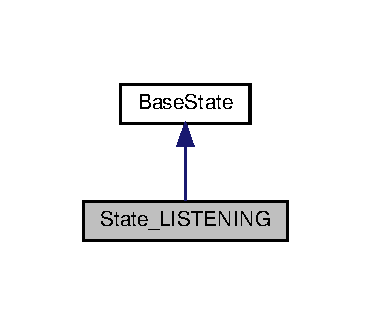
\includegraphics[width=178pt]{class_state___l_i_s_t_e_n_i_n_g__coll__graph}
\end{center}
\end{figure}
\subsection*{Public Member Functions}
\begin{DoxyCompactItemize}
\item 
virtual void \hyperlink{class_state___l_i_s_t_e_n_i_n_g_af77af4f01ff6fde1f64b133c5fa61cb8}{drive} (\hyperlink{class_state_machine}{State\+Machine} $\ast$m)
\begin{DoxyCompactList}\small\item\em Switch to driving mode. \end{DoxyCompactList}\item 
virtual void \hyperlink{class_state___l_i_s_t_e_n_i_n_g_a0063dbc4d0cc0712e4a69e67a452f92b}{listen} (\hyperlink{class_state_machine}{State\+Machine} $\ast$m)
\begin{DoxyCompactList}\small\item\em Don\textquotesingle{}t do anything on command listen. \end{DoxyCompactList}\item 
virtual void \hyperlink{class_state___l_i_s_t_e_n_i_n_g_ab6eba322cb293ec2b693f48260f72751}{go\+\_\+to} (\hyperlink{class_state_machine}{State\+Machine} $\ast$m, string target)
\begin{DoxyCompactList}\small\item\em Switch to go\+\_\+to mode. \end{DoxyCompactList}\item 
virtual void \hyperlink{class_state___l_i_s_t_e_n_i_n_g_a780b6f499710282279e60c7e48cd6611}{label} (\hyperlink{class_state_machine}{State\+Machine} $\ast$m, string label)
\begin{DoxyCompactList}\small\item\em Call label service. \end{DoxyCompactList}\item 
virtual void \hyperlink{class_state___l_i_s_t_e_n_i_n_g_a673b6c2cd73588f9db6b252c5e0d6d60}{goal\+\_\+reached} (\hyperlink{class_state_machine}{State\+Machine} $\ast$m)
\begin{DoxyCompactList}\small\item\em Don\textquotesingle{}t do anything when goal reached is received. \end{DoxyCompactList}\end{DoxyCompactItemize}


\subsection{Detailed Description}
State class for the mode, when the system is listening to voice commands. 

Robot is not moving in this mode! 

Definition at line 12 of file State\+\_\+\+L\+I\+S\+T\+E\+N\+I\+N\+G.\+h.



\subsection{Member Function Documentation}
\mbox{\Hypertarget{class_state___l_i_s_t_e_n_i_n_g_af77af4f01ff6fde1f64b133c5fa61cb8}\label{class_state___l_i_s_t_e_n_i_n_g_af77af4f01ff6fde1f64b133c5fa61cb8}} 
\index{State\+\_\+\+L\+I\+S\+T\+E\+N\+I\+NG@{State\+\_\+\+L\+I\+S\+T\+E\+N\+I\+NG}!drive@{drive}}
\index{drive@{drive}!State\+\_\+\+L\+I\+S\+T\+E\+N\+I\+NG@{State\+\_\+\+L\+I\+S\+T\+E\+N\+I\+NG}}
\subsubsection{\texorpdfstring{drive()}{drive()}}
{\footnotesize\ttfamily void State\+\_\+\+L\+I\+S\+T\+E\+N\+I\+N\+G\+::drive (\begin{DoxyParamCaption}\item[{\hyperlink{class_state_machine}{State\+Machine} $\ast$}]{m }\end{DoxyParamCaption})\hspace{0.3cm}{\ttfamily [virtual]}}



Switch to driving mode. 



Implements \hyperlink{class_base_state_a398bc67a0353c3e8da1597dbdbbba2cc}{Base\+State}.



Definition at line 10 of file State\+\_\+\+L\+I\+S\+T\+E\+N\+I\+N\+G.\+cpp.

\mbox{\Hypertarget{class_state___l_i_s_t_e_n_i_n_g_ab6eba322cb293ec2b693f48260f72751}\label{class_state___l_i_s_t_e_n_i_n_g_ab6eba322cb293ec2b693f48260f72751}} 
\index{State\+\_\+\+L\+I\+S\+T\+E\+N\+I\+NG@{State\+\_\+\+L\+I\+S\+T\+E\+N\+I\+NG}!go\+\_\+to@{go\+\_\+to}}
\index{go\+\_\+to@{go\+\_\+to}!State\+\_\+\+L\+I\+S\+T\+E\+N\+I\+NG@{State\+\_\+\+L\+I\+S\+T\+E\+N\+I\+NG}}
\subsubsection{\texorpdfstring{go\+\_\+to()}{go\_to()}}
{\footnotesize\ttfamily void State\+\_\+\+L\+I\+S\+T\+E\+N\+I\+N\+G\+::go\+\_\+to (\begin{DoxyParamCaption}\item[{\hyperlink{class_state_machine}{State\+Machine} $\ast$}]{m,  }\item[{string}]{target }\end{DoxyParamCaption})\hspace{0.3cm}{\ttfamily [virtual]}}



Switch to go\+\_\+to mode. 



Implements \hyperlink{class_base_state_a6acb02c9d6b3e54602e163dc1848ac3a}{Base\+State}.



Definition at line 28 of file State\+\_\+\+L\+I\+S\+T\+E\+N\+I\+N\+G.\+cpp.

\mbox{\Hypertarget{class_state___l_i_s_t_e_n_i_n_g_a673b6c2cd73588f9db6b252c5e0d6d60}\label{class_state___l_i_s_t_e_n_i_n_g_a673b6c2cd73588f9db6b252c5e0d6d60}} 
\index{State\+\_\+\+L\+I\+S\+T\+E\+N\+I\+NG@{State\+\_\+\+L\+I\+S\+T\+E\+N\+I\+NG}!goal\+\_\+reached@{goal\+\_\+reached}}
\index{goal\+\_\+reached@{goal\+\_\+reached}!State\+\_\+\+L\+I\+S\+T\+E\+N\+I\+NG@{State\+\_\+\+L\+I\+S\+T\+E\+N\+I\+NG}}
\subsubsection{\texorpdfstring{goal\+\_\+reached()}{goal\_reached()}}
{\footnotesize\ttfamily void State\+\_\+\+L\+I\+S\+T\+E\+N\+I\+N\+G\+::goal\+\_\+reached (\begin{DoxyParamCaption}\item[{\hyperlink{class_state_machine}{State\+Machine} $\ast$}]{m }\end{DoxyParamCaption})\hspace{0.3cm}{\ttfamily [virtual]}}



Don\textquotesingle{}t do anything when goal reached is received. 



Implements \hyperlink{class_base_state_aafa71e762d651f1f5a1f7a6decd0d3b5}{Base\+State}.



Definition at line 55 of file State\+\_\+\+L\+I\+S\+T\+E\+N\+I\+N\+G.\+cpp.

\mbox{\Hypertarget{class_state___l_i_s_t_e_n_i_n_g_a780b6f499710282279e60c7e48cd6611}\label{class_state___l_i_s_t_e_n_i_n_g_a780b6f499710282279e60c7e48cd6611}} 
\index{State\+\_\+\+L\+I\+S\+T\+E\+N\+I\+NG@{State\+\_\+\+L\+I\+S\+T\+E\+N\+I\+NG}!label@{label}}
\index{label@{label}!State\+\_\+\+L\+I\+S\+T\+E\+N\+I\+NG@{State\+\_\+\+L\+I\+S\+T\+E\+N\+I\+NG}}
\subsubsection{\texorpdfstring{label()}{label()}}
{\footnotesize\ttfamily void State\+\_\+\+L\+I\+S\+T\+E\+N\+I\+N\+G\+::label (\begin{DoxyParamCaption}\item[{\hyperlink{class_state_machine}{State\+Machine} $\ast$}]{m,  }\item[{string}]{label }\end{DoxyParamCaption})\hspace{0.3cm}{\ttfamily [virtual]}}



Call label service. 



Implements \hyperlink{class_base_state_a9b21ace3d89308945fdecd81b34d3919}{Base\+State}.



Definition at line 39 of file State\+\_\+\+L\+I\+S\+T\+E\+N\+I\+N\+G.\+cpp.

\mbox{\Hypertarget{class_state___l_i_s_t_e_n_i_n_g_a0063dbc4d0cc0712e4a69e67a452f92b}\label{class_state___l_i_s_t_e_n_i_n_g_a0063dbc4d0cc0712e4a69e67a452f92b}} 
\index{State\+\_\+\+L\+I\+S\+T\+E\+N\+I\+NG@{State\+\_\+\+L\+I\+S\+T\+E\+N\+I\+NG}!listen@{listen}}
\index{listen@{listen}!State\+\_\+\+L\+I\+S\+T\+E\+N\+I\+NG@{State\+\_\+\+L\+I\+S\+T\+E\+N\+I\+NG}}
\subsubsection{\texorpdfstring{listen()}{listen()}}
{\footnotesize\ttfamily void State\+\_\+\+L\+I\+S\+T\+E\+N\+I\+N\+G\+::listen (\begin{DoxyParamCaption}\item[{\hyperlink{class_state_machine}{State\+Machine} $\ast$}]{m }\end{DoxyParamCaption})\hspace{0.3cm}{\ttfamily [virtual]}}



Don\textquotesingle{}t do anything on command listen. 



Implements \hyperlink{class_base_state_ac65db46601f60cd025ff058dae117d7c}{Base\+State}.



Definition at line 20 of file State\+\_\+\+L\+I\+S\+T\+E\+N\+I\+N\+G.\+cpp.



The documentation for this class was generated from the following files\+:\begin{DoxyCompactItemize}
\item 
catkin\+\_\+ws/src/labeled\+\_\+slam/include/labeled\+\_\+slam/\+State\+Machine/\hyperlink{_state___l_i_s_t_e_n_i_n_g_8h}{State\+\_\+\+L\+I\+S\+T\+E\+N\+I\+N\+G.\+h}\item 
catkin\+\_\+ws/src/labeled\+\_\+slam/src/\+State\+Machine/\hyperlink{_state___l_i_s_t_e_n_i_n_g_8cpp}{State\+\_\+\+L\+I\+S\+T\+E\+N\+I\+N\+G.\+cpp}\end{DoxyCompactItemize}

\hypertarget{class_state_machine}{}\section{State\+Machine Class Reference}
\label{class_state_machine}\index{State\+Machine@{State\+Machine}}


Implements the interface for the labeled\+\_\+slam state machine.  




{\ttfamily \#include $<$State\+Machine.\+h$>$}

\subsection*{Public Member Functions}
\begin{DoxyCompactItemize}
\item 
\hyperlink{class_state_machine_aa4732b2706c581cb8aac47674b52a8b5}{State\+Machine} (ros\+::\+Service\+Client $\ast$client\+\_\+set\+\_\+goal, ros\+::\+Service\+Client $\ast$client\+\_\+set\+\_\+label, ros\+::\+Service\+Client $\ast$client\+\_\+activate\+\_\+path\+\_\+following, ros\+::\+Service\+Client $\ast$client\+\_\+activate\+\_\+driving)
\begin{DoxyCompactList}\small\item\em Constructor. \end{DoxyCompactList}\item 
\hyperlink{class_state_machine_a93d66cb2a89b186789d655a08b02674e}{$\sim$\+State\+Machine} ()
\begin{DoxyCompactList}\small\item\em Destructor. \end{DoxyCompactList}\item 
void \hyperlink{class_state_machine_a0d90a952683cb15f30bfbaea63ff2e10}{callback\+\_\+command} (const labeled\+\_\+slam\+::\+Command\+::\+Const\+Ptr \&\hyperlink{velocity__forwarder_8cpp_aba2f97176e275688941f5c2a40324b8a}{msg})
\begin{DoxyCompactList}\small\item\em Callback function for text\+\_\+command subscriber. \end{DoxyCompactList}\item 
void \hyperlink{class_state_machine_ae36de4ee8784f1ef63e5721aed3465fc}{callback\+\_\+goal\+\_\+reached} (const std\+\_\+msgs\+::\+Bool\+::\+Const\+Ptr \&\hyperlink{velocity__forwarder_8cpp_aba2f97176e275688941f5c2a40324b8a}{msg})
\begin{DoxyCompactList}\small\item\em Callback function for goal\+\_\+reached subscriber. \end{DoxyCompactList}\end{DoxyCompactItemize}
\subsection*{Friends}
\begin{DoxyCompactItemize}
\item 
class \hyperlink{class_state_machine_a9f3d690f79a1c7f54e4417a8a3dfab55}{State\+\_\+\+D\+R\+I\+V\+I\+NG}
\item 
class \hyperlink{class_state_machine_a6309eb5fa74ee5fdbbe99598c54aa8ef}{State\+\_\+\+L\+I\+S\+T\+E\+N\+I\+NG}
\item 
class \hyperlink{class_state_machine_ae1f479386d109e891cf95b71a1fa9d38}{State\+\_\+\+G\+O\+\_\+\+TO}
\end{DoxyCompactItemize}


\subsection{Detailed Description}
Implements the interface for the labeled\+\_\+slam state machine. 

Uses the c++ \textquotesingle{}State\textquotesingle{}-\/pattern 

Definition at line 41 of file State\+Machine.\+h.



\subsection{Constructor \& Destructor Documentation}
\mbox{\Hypertarget{class_state_machine_aa4732b2706c581cb8aac47674b52a8b5}\label{class_state_machine_aa4732b2706c581cb8aac47674b52a8b5}} 
\index{State\+Machine@{State\+Machine}!State\+Machine@{State\+Machine}}
\index{State\+Machine@{State\+Machine}!State\+Machine@{State\+Machine}}
\subsubsection{\texorpdfstring{State\+Machine()}{StateMachine()}}
{\footnotesize\ttfamily State\+Machine\+::\+State\+Machine (\begin{DoxyParamCaption}\item[{ros\+::\+Service\+Client $\ast$}]{client\+\_\+set\+\_\+goal,  }\item[{ros\+::\+Service\+Client $\ast$}]{client\+\_\+set\+\_\+label,  }\item[{ros\+::\+Service\+Client $\ast$}]{client\+\_\+activate\+\_\+path\+\_\+following,  }\item[{ros\+::\+Service\+Client $\ast$}]{client\+\_\+activate\+\_\+driving }\end{DoxyParamCaption})}



Constructor. 

Constructor of \hyperlink{class_state_machine}{State\+Machine} Class. 

Definition at line 11 of file State\+Machine.\+cpp.

\mbox{\Hypertarget{class_state_machine_a93d66cb2a89b186789d655a08b02674e}\label{class_state_machine_a93d66cb2a89b186789d655a08b02674e}} 
\index{State\+Machine@{State\+Machine}!````~State\+Machine@{$\sim$\+State\+Machine}}
\index{````~State\+Machine@{$\sim$\+State\+Machine}!State\+Machine@{State\+Machine}}
\subsubsection{\texorpdfstring{$\sim$\+State\+Machine()}{~StateMachine()}}
{\footnotesize\ttfamily State\+Machine\+::$\sim$\+State\+Machine (\begin{DoxyParamCaption}{ }\end{DoxyParamCaption})}



Destructor. 

Destructor of \hyperlink{class_state_machine}{State\+Machine} Class. 

Definition at line 26 of file State\+Machine.\+cpp.



\subsection{Member Function Documentation}
\mbox{\Hypertarget{class_state_machine_a0d90a952683cb15f30bfbaea63ff2e10}\label{class_state_machine_a0d90a952683cb15f30bfbaea63ff2e10}} 
\index{State\+Machine@{State\+Machine}!callback\+\_\+command@{callback\+\_\+command}}
\index{callback\+\_\+command@{callback\+\_\+command}!State\+Machine@{State\+Machine}}
\subsubsection{\texorpdfstring{callback\+\_\+command()}{callback\_command()}}
{\footnotesize\ttfamily void State\+Machine\+::callback\+\_\+command (\begin{DoxyParamCaption}\item[{const labeled\+\_\+slam\+::\+Command\+::\+Const\+Ptr \&}]{msg }\end{DoxyParamCaption})}



Callback function for text\+\_\+command subscriber. 

Callback-\/function interpreting command from command-\/recognition node.

Allowed commands are \char`\"{}drive\char`\"{}, \char`\"{}go to\char`\"{}, \char`\"{}label\char`\"{}, \char`\"{}listen\char`\"{} commands go\+\_\+to and label are using an argument. For the other commands, the argument is just ignored. According function of the state\+\_\+member are called on each command Depending on the true object-\/type in the state\+\_\+-\/variable, the function of one specific state is called (P\+O\+L\+Y\+M\+O\+R\+P\+H\+I\+S\+M!) 

Definition at line 41 of file State\+Machine.\+cpp.

\mbox{\Hypertarget{class_state_machine_ae36de4ee8784f1ef63e5721aed3465fc}\label{class_state_machine_ae36de4ee8784f1ef63e5721aed3465fc}} 
\index{State\+Machine@{State\+Machine}!callback\+\_\+goal\+\_\+reached@{callback\+\_\+goal\+\_\+reached}}
\index{callback\+\_\+goal\+\_\+reached@{callback\+\_\+goal\+\_\+reached}!State\+Machine@{State\+Machine}}
\subsubsection{\texorpdfstring{callback\+\_\+goal\+\_\+reached()}{callback\_goal\_reached()}}
{\footnotesize\ttfamily void State\+Machine\+::callback\+\_\+goal\+\_\+reached (\begin{DoxyParamCaption}\item[{const std\+\_\+msgs\+::\+Bool\+::\+Const\+Ptr \&}]{msg }\end{DoxyParamCaption})}



Callback function for goal\+\_\+reached subscriber. 

Callback-\/function for the subscribed topic goal\+\_\+reached. 

Definition at line 72 of file State\+Machine.\+cpp.



\subsection{Friends And Related Function Documentation}
\mbox{\Hypertarget{class_state_machine_a9f3d690f79a1c7f54e4417a8a3dfab55}\label{class_state_machine_a9f3d690f79a1c7f54e4417a8a3dfab55}} 
\index{State\+Machine@{State\+Machine}!State\+\_\+\+D\+R\+I\+V\+I\+NG@{State\+\_\+\+D\+R\+I\+V\+I\+NG}}
\index{State\+\_\+\+D\+R\+I\+V\+I\+NG@{State\+\_\+\+D\+R\+I\+V\+I\+NG}!State\+Machine@{State\+Machine}}
\subsubsection{\texorpdfstring{State\+\_\+\+D\+R\+I\+V\+I\+NG}{State\_DRIVING}}
{\footnotesize\ttfamily friend class \hyperlink{class_state___d_r_i_v_i_n_g}{State\+\_\+\+D\+R\+I\+V\+I\+NG}\hspace{0.3cm}{\ttfamily [friend]}}



Definition at line 71 of file State\+Machine.\+h.

\mbox{\Hypertarget{class_state_machine_ae1f479386d109e891cf95b71a1fa9d38}\label{class_state_machine_ae1f479386d109e891cf95b71a1fa9d38}} 
\index{State\+Machine@{State\+Machine}!State\+\_\+\+G\+O\+\_\+\+TO@{State\+\_\+\+G\+O\+\_\+\+TO}}
\index{State\+\_\+\+G\+O\+\_\+\+TO@{State\+\_\+\+G\+O\+\_\+\+TO}!State\+Machine@{State\+Machine}}
\subsubsection{\texorpdfstring{State\+\_\+\+G\+O\+\_\+\+TO}{State\_GO\_TO}}
{\footnotesize\ttfamily friend class \hyperlink{class_state___g_o___t_o}{State\+\_\+\+G\+O\+\_\+\+TO}\hspace{0.3cm}{\ttfamily [friend]}}



Definition at line 73 of file State\+Machine.\+h.

\mbox{\Hypertarget{class_state_machine_a6309eb5fa74ee5fdbbe99598c54aa8ef}\label{class_state_machine_a6309eb5fa74ee5fdbbe99598c54aa8ef}} 
\index{State\+Machine@{State\+Machine}!State\+\_\+\+L\+I\+S\+T\+E\+N\+I\+NG@{State\+\_\+\+L\+I\+S\+T\+E\+N\+I\+NG}}
\index{State\+\_\+\+L\+I\+S\+T\+E\+N\+I\+NG@{State\+\_\+\+L\+I\+S\+T\+E\+N\+I\+NG}!State\+Machine@{State\+Machine}}
\subsubsection{\texorpdfstring{State\+\_\+\+L\+I\+S\+T\+E\+N\+I\+NG}{State\_LISTENING}}
{\footnotesize\ttfamily friend class \hyperlink{class_state___l_i_s_t_e_n_i_n_g}{State\+\_\+\+L\+I\+S\+T\+E\+N\+I\+NG}\hspace{0.3cm}{\ttfamily [friend]}}



Definition at line 72 of file State\+Machine.\+h.



The documentation for this class was generated from the following files\+:\begin{DoxyCompactItemize}
\item 
catkin\+\_\+ws/src/labeled\+\_\+slam/include/labeled\+\_\+slam/\+State\+Machine/\hyperlink{_state_machine_8h}{State\+Machine.\+h}\item 
catkin\+\_\+ws/src/labeled\+\_\+slam/src/\+State\+Machine/\hyperlink{_state_machine_8cpp}{State\+Machine.\+cpp}\end{DoxyCompactItemize}

\chapter{File Documentation}
\hypertarget{_base_state_8h}{}\section{catkin\+\_\+ws/src/labeled\+\_\+slam/include/labeled\+\_\+slam/\+State\+Machine/\+Base\+State.h File Reference}
\label{_base_state_8h}\index{catkin\+\_\+ws/src/labeled\+\_\+slam/include/labeled\+\_\+slam/\+State\+Machine/\+Base\+State.\+h@{catkin\+\_\+ws/src/labeled\+\_\+slam/include/labeled\+\_\+slam/\+State\+Machine/\+Base\+State.\+h}}
{\ttfamily \#include \char`\"{}ros/ros.\+h\char`\"{}}\newline
{\ttfamily \#include $<$string$>$}\newline
Include dependency graph for Base\+State.\+h\+:\nopagebreak
\begin{figure}[H]
\begin{center}
\leavevmode
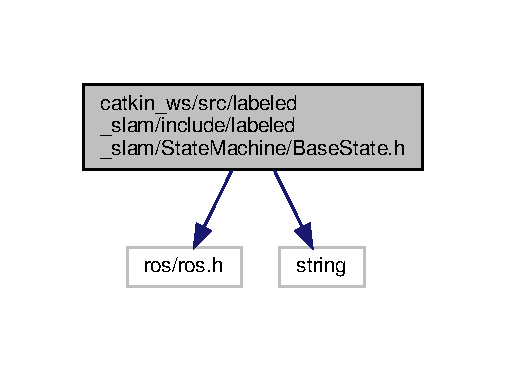
\includegraphics[width=243pt]{_base_state_8h__incl}
\end{center}
\end{figure}
This graph shows which files directly or indirectly include this file\+:\nopagebreak
\begin{figure}[H]
\begin{center}
\leavevmode
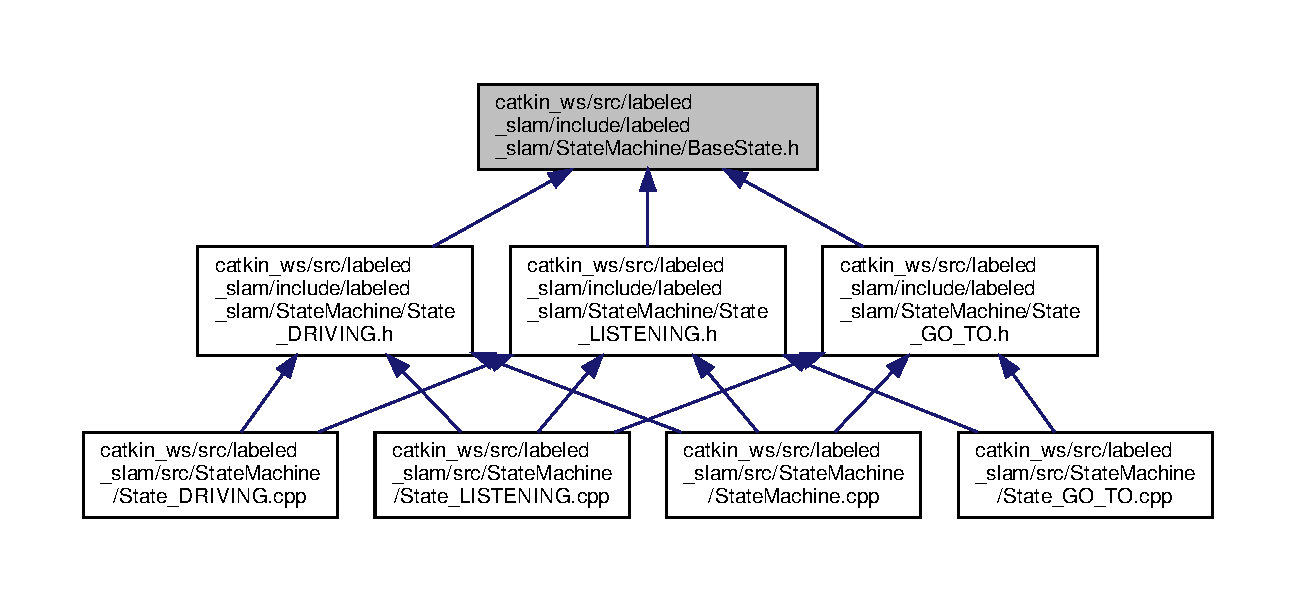
\includegraphics[width=350pt]{_base_state_8h__dep__incl}
\end{center}
\end{figure}
\subsection*{Classes}
\begin{DoxyCompactItemize}
\item 
class \hyperlink{class_base_state}{Base\+State}
\begin{DoxyCompactList}\small\item\em Base class for all the specific state classes. Contains public interface of all derived classes. \end{DoxyCompactList}\end{DoxyCompactItemize}

\hypertarget{_state___d_r_i_v_i_n_g_8h}{}\section{catkin\+\_\+ws/src/labeled\+\_\+slam/include/labeled\+\_\+slam/\+State\+Machine/\+State\+\_\+\+D\+R\+I\+V\+I\+NG.h File Reference}
\label{_state___d_r_i_v_i_n_g_8h}\index{catkin\+\_\+ws/src/labeled\+\_\+slam/include/labeled\+\_\+slam/\+State\+Machine/\+State\+\_\+\+D\+R\+I\+V\+I\+N\+G.\+h@{catkin\+\_\+ws/src/labeled\+\_\+slam/include/labeled\+\_\+slam/\+State\+Machine/\+State\+\_\+\+D\+R\+I\+V\+I\+N\+G.\+h}}
{\ttfamily \#include \char`\"{}Base\+State.\+h\char`\"{}}\newline
Include dependency graph for State\+\_\+\+D\+R\+I\+V\+I\+N\+G.\+h\+:\nopagebreak
\begin{figure}[H]
\begin{center}
\leavevmode
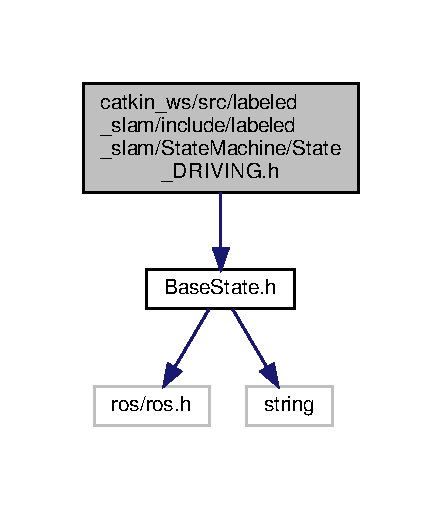
\includegraphics[width=212pt]{_state___d_r_i_v_i_n_g_8h__incl}
\end{center}
\end{figure}
This graph shows which files directly or indirectly include this file\+:\nopagebreak
\begin{figure}[H]
\begin{center}
\leavevmode
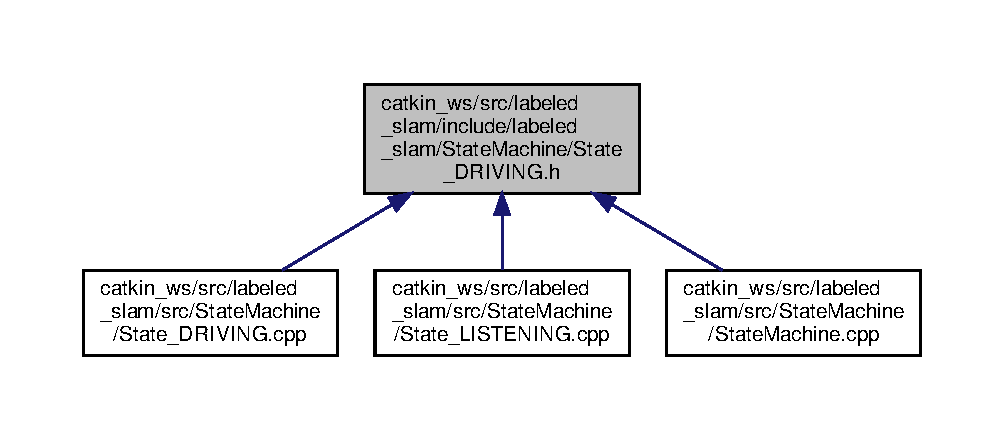
\includegraphics[width=350pt]{_state___d_r_i_v_i_n_g_8h__dep__incl}
\end{center}
\end{figure}
\subsection*{Classes}
\begin{DoxyCompactItemize}
\item 
class \hyperlink{class_state___d_r_i_v_i_n_g}{State\+\_\+\+D\+R\+I\+V\+I\+NG}
\begin{DoxyCompactList}\small\item\em State class for the mode, when the robot is controlled manually using the smartwatch. \end{DoxyCompactList}\end{DoxyCompactItemize}

\hypertarget{_state___g_o___t_o_8h}{}\section{catkin\+\_\+ws/src/labeled\+\_\+slam/include/labeled\+\_\+slam/\+State\+Machine/\+State\+\_\+\+G\+O\+\_\+\+TO.h File Reference}
\label{_state___g_o___t_o_8h}\index{catkin\+\_\+ws/src/labeled\+\_\+slam/include/labeled\+\_\+slam/\+State\+Machine/\+State\+\_\+\+G\+O\+\_\+\+T\+O.\+h@{catkin\+\_\+ws/src/labeled\+\_\+slam/include/labeled\+\_\+slam/\+State\+Machine/\+State\+\_\+\+G\+O\+\_\+\+T\+O.\+h}}
{\ttfamily \#include \char`\"{}Base\+State.\+h\char`\"{}}\newline
Include dependency graph for State\+\_\+\+G\+O\+\_\+\+T\+O.\+h\+:\nopagebreak
\begin{figure}[H]
\begin{center}
\leavevmode
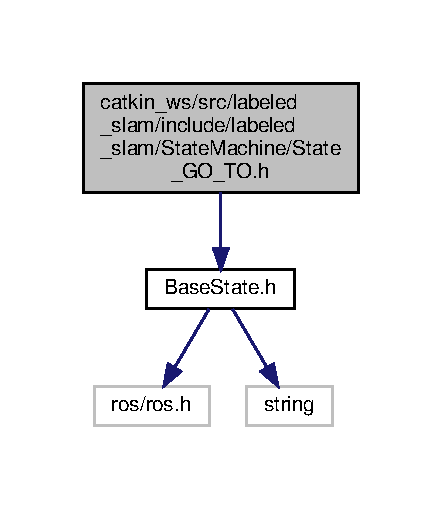
\includegraphics[width=212pt]{_state___g_o___t_o_8h__incl}
\end{center}
\end{figure}
This graph shows which files directly or indirectly include this file\+:\nopagebreak
\begin{figure}[H]
\begin{center}
\leavevmode
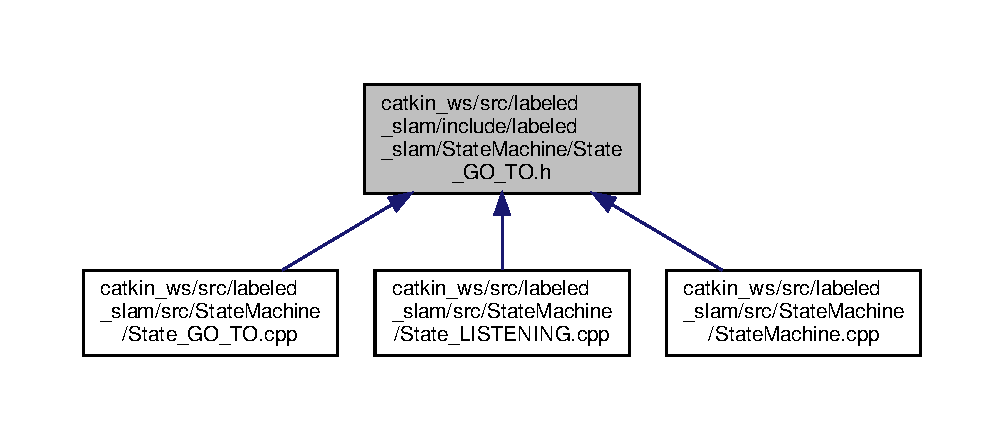
\includegraphics[width=350pt]{_state___g_o___t_o_8h__dep__incl}
\end{center}
\end{figure}
\subsection*{Classes}
\begin{DoxyCompactItemize}
\item 
class \hyperlink{class_state___g_o___t_o}{State\+\_\+\+G\+O\+\_\+\+TO}
\begin{DoxyCompactList}\small\item\em State class for the mode, when the system is following a path towards a target. \end{DoxyCompactList}\end{DoxyCompactItemize}

\hypertarget{_state___l_i_s_t_e_n_i_n_g_8h}{}\section{catkin\+\_\+ws/src/labeled\+\_\+slam/include/labeled\+\_\+slam/\+State\+Machine/\+State\+\_\+\+L\+I\+S\+T\+E\+N\+I\+NG.h File Reference}
\label{_state___l_i_s_t_e_n_i_n_g_8h}\index{catkin\+\_\+ws/src/labeled\+\_\+slam/include/labeled\+\_\+slam/\+State\+Machine/\+State\+\_\+\+L\+I\+S\+T\+E\+N\+I\+N\+G.\+h@{catkin\+\_\+ws/src/labeled\+\_\+slam/include/labeled\+\_\+slam/\+State\+Machine/\+State\+\_\+\+L\+I\+S\+T\+E\+N\+I\+N\+G.\+h}}
{\ttfamily \#include \char`\"{}Base\+State.\+h\char`\"{}}\newline
Include dependency graph for State\+\_\+\+L\+I\+S\+T\+E\+N\+I\+N\+G.\+h\+:
\nopagebreak
\begin{figure}[H]
\begin{center}
\leavevmode
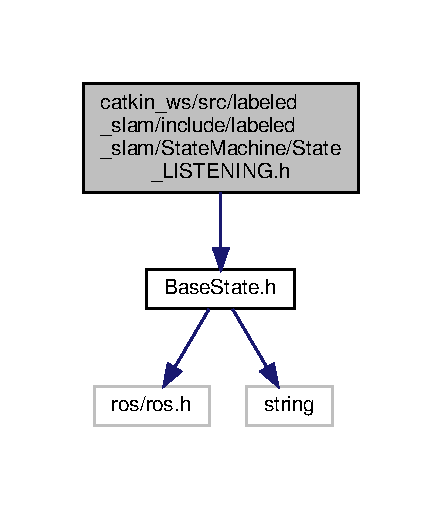
\includegraphics[width=212pt]{_state___l_i_s_t_e_n_i_n_g_8h__incl}
\end{center}
\end{figure}
This graph shows which files directly or indirectly include this file\+:
\nopagebreak
\begin{figure}[H]
\begin{center}
\leavevmode
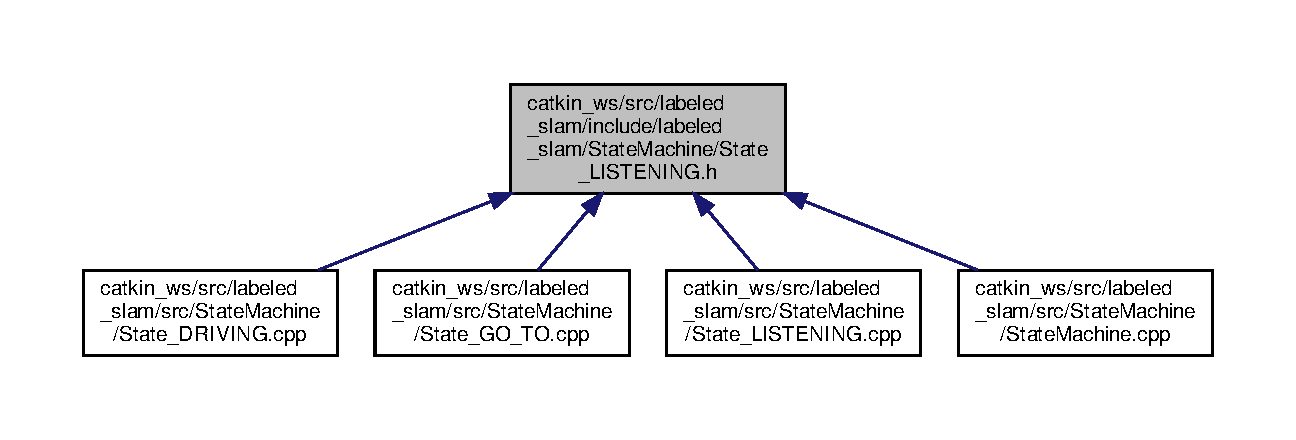
\includegraphics[width=350pt]{_state___l_i_s_t_e_n_i_n_g_8h__dep__incl}
\end{center}
\end{figure}
\subsection*{Classes}
\begin{DoxyCompactItemize}
\item 
class \hyperlink{class_state___l_i_s_t_e_n_i_n_g}{State\+\_\+\+L\+I\+S\+T\+E\+N\+I\+NG}
\begin{DoxyCompactList}\small\item\em State class for the mode, when the system is listening to voice commands. \end{DoxyCompactList}\end{DoxyCompactItemize}

\hypertarget{_state_machine_8h}{}\section{catkin\+\_\+ws/src/labeled\+\_\+slam/include/labeled\+\_\+slam/\+State\+Machine/\+State\+Machine.h File Reference}
\label{_state_machine_8h}\index{catkin\+\_\+ws/src/labeled\+\_\+slam/include/labeled\+\_\+slam/\+State\+Machine/\+State\+Machine.\+h@{catkin\+\_\+ws/src/labeled\+\_\+slam/include/labeled\+\_\+slam/\+State\+Machine/\+State\+Machine.\+h}}
{\ttfamily \#include \char`\"{}ros/ros.\+h\char`\"{}}\newline
{\ttfamily \#include \char`\"{}ros/time.\+h\char`\"{}}\newline
{\ttfamily \#include \char`\"{}labeled\+\_\+slam/\+Command.\+h\char`\"{}}\newline
{\ttfamily \#include \char`\"{}std\+\_\+srvs/\+Set\+Bool.\+h\char`\"{}}\newline
{\ttfamily \#include \char`\"{}std\+\_\+msgs/\+Bool.\+h\char`\"{}}\newline
{\ttfamily \#include \char`\"{}rtabmap\+\_\+ros/\+Set\+Goal.\+h\char`\"{}}\newline
{\ttfamily \#include \char`\"{}rtabmap\+\_\+ros/\+Set\+Label.\+h\char`\"{}}\newline
Include dependency graph for State\+Machine.\+h\+:
\nopagebreak
\begin{figure}[H]
\begin{center}
\leavevmode
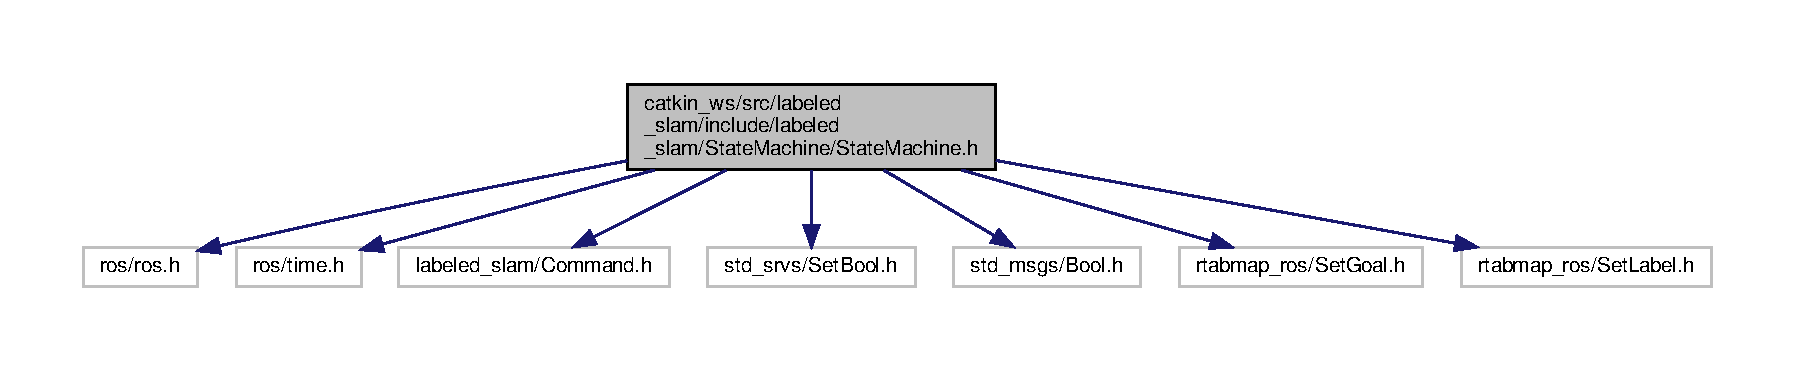
\includegraphics[width=350pt]{_state_machine_8h__incl}
\end{center}
\end{figure}
This graph shows which files directly or indirectly include this file\+:
\nopagebreak
\begin{figure}[H]
\begin{center}
\leavevmode
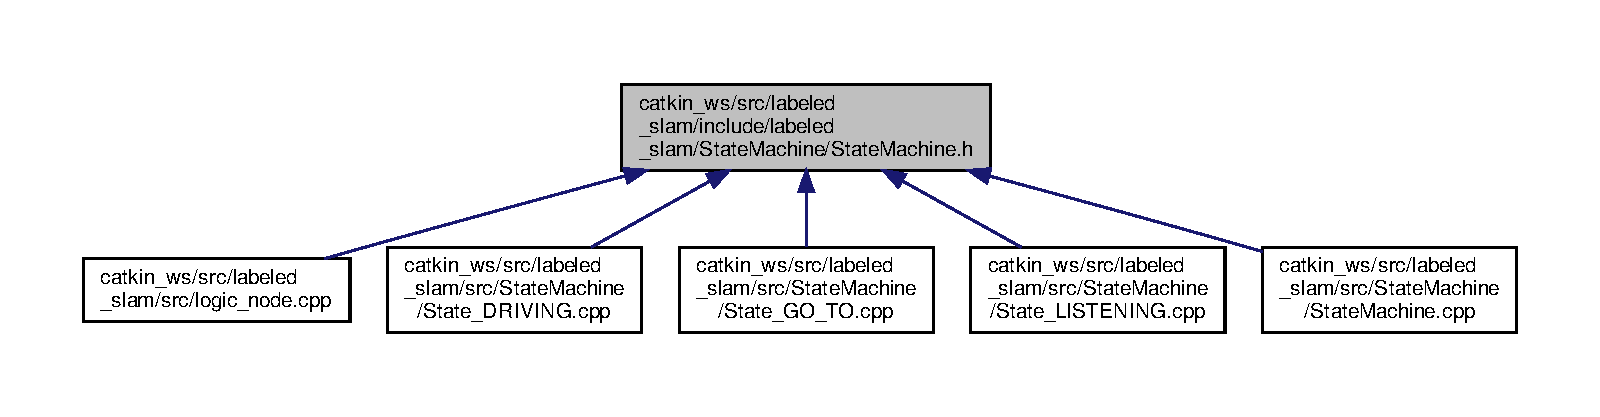
\includegraphics[width=350pt]{_state_machine_8h__dep__incl}
\end{center}
\end{figure}
\subsection*{Classes}
\begin{DoxyCompactItemize}
\item 
class \hyperlink{class_state_machine}{State\+Machine}
\begin{DoxyCompactList}\small\item\em Implements the interface for the labeled\+\_\+slam state machine. \end{DoxyCompactList}\end{DoxyCompactItemize}
\subsection*{Macros}
\begin{DoxyCompactItemize}
\item 
\#define \hyperlink{_state_machine_8h_a6195ed35f32426bdf073b3a3b8dda6e3}{S\+R\+V\+\_\+\+T\+Y\+P\+E\+\_\+\+S\+E\+T\+\_\+\+G\+O\+AL}~rtabmap\+\_\+ros\+::\+Set\+Goal
\item 
\#define \hyperlink{_state_machine_8h_ab537bf4836228673e13fbcfa66678ed9}{S\+R\+V\+\_\+\+T\+Y\+P\+E\+\_\+\+S\+E\+T\+\_\+\+L\+A\+B\+EL}~rtabmap\+\_\+ros\+::\+Set\+Label
\end{DoxyCompactItemize}


\subsection{Macro Definition Documentation}
\mbox{\Hypertarget{_state_machine_8h_a6195ed35f32426bdf073b3a3b8dda6e3}\label{_state_machine_8h_a6195ed35f32426bdf073b3a3b8dda6e3}} 
\index{State\+Machine.\+h@{State\+Machine.\+h}!S\+R\+V\+\_\+\+T\+Y\+P\+E\+\_\+\+S\+E\+T\+\_\+\+G\+O\+AL@{S\+R\+V\+\_\+\+T\+Y\+P\+E\+\_\+\+S\+E\+T\+\_\+\+G\+O\+AL}}
\index{S\+R\+V\+\_\+\+T\+Y\+P\+E\+\_\+\+S\+E\+T\+\_\+\+G\+O\+AL@{S\+R\+V\+\_\+\+T\+Y\+P\+E\+\_\+\+S\+E\+T\+\_\+\+G\+O\+AL}!State\+Machine.\+h@{State\+Machine.\+h}}
\subsubsection{\texorpdfstring{S\+R\+V\+\_\+\+T\+Y\+P\+E\+\_\+\+S\+E\+T\+\_\+\+G\+O\+AL}{SRV\_TYPE\_SET\_GOAL}}
{\footnotesize\ttfamily \#define S\+R\+V\+\_\+\+T\+Y\+P\+E\+\_\+\+S\+E\+T\+\_\+\+G\+O\+AL~rtabmap\+\_\+ros\+::\+Set\+Goal}



Definition at line 22 of file State\+Machine.\+h.

\mbox{\Hypertarget{_state_machine_8h_ab537bf4836228673e13fbcfa66678ed9}\label{_state_machine_8h_ab537bf4836228673e13fbcfa66678ed9}} 
\index{State\+Machine.\+h@{State\+Machine.\+h}!S\+R\+V\+\_\+\+T\+Y\+P\+E\+\_\+\+S\+E\+T\+\_\+\+L\+A\+B\+EL@{S\+R\+V\+\_\+\+T\+Y\+P\+E\+\_\+\+S\+E\+T\+\_\+\+L\+A\+B\+EL}}
\index{S\+R\+V\+\_\+\+T\+Y\+P\+E\+\_\+\+S\+E\+T\+\_\+\+L\+A\+B\+EL@{S\+R\+V\+\_\+\+T\+Y\+P\+E\+\_\+\+S\+E\+T\+\_\+\+L\+A\+B\+EL}!State\+Machine.\+h@{State\+Machine.\+h}}
\subsubsection{\texorpdfstring{S\+R\+V\+\_\+\+T\+Y\+P\+E\+\_\+\+S\+E\+T\+\_\+\+L\+A\+B\+EL}{SRV\_TYPE\_SET\_LABEL}}
{\footnotesize\ttfamily \#define S\+R\+V\+\_\+\+T\+Y\+P\+E\+\_\+\+S\+E\+T\+\_\+\+L\+A\+B\+EL~rtabmap\+\_\+ros\+::\+Set\+Label}



Definition at line 23 of file State\+Machine.\+h.


\hypertarget{activator1_8cpp}{}\section{catkin\+\_\+ws/src/labeled\+\_\+slam/src/activator1.cpp File Reference}
\label{activator1_8cpp}\index{catkin\+\_\+ws/src/labeled\+\_\+slam/src/activator1.\+cpp@{catkin\+\_\+ws/src/labeled\+\_\+slam/src/activator1.\+cpp}}
{\ttfamily \#include $<$sstream$>$}\newline
{\ttfamily \#include $<$stdlib.\+h$>$}\newline
{\ttfamily \#include \char`\"{}ros/ros.\+h\char`\"{}}\newline
{\ttfamily \#include \char`\"{}std\+\_\+msgs/\+Bool.\+h\char`\"{}}\newline
{\ttfamily \#include \char`\"{}std\+\_\+srvs/\+Set\+Bool.\+h\char`\"{}}\newline
{\ttfamily \#include \char`\"{}geometry\+\_\+msgs/\+Twist.\+h\char`\"{}}\newline
Include dependency graph for activator1.\+cpp\+:\nopagebreak
\begin{figure}[H]
\begin{center}
\leavevmode
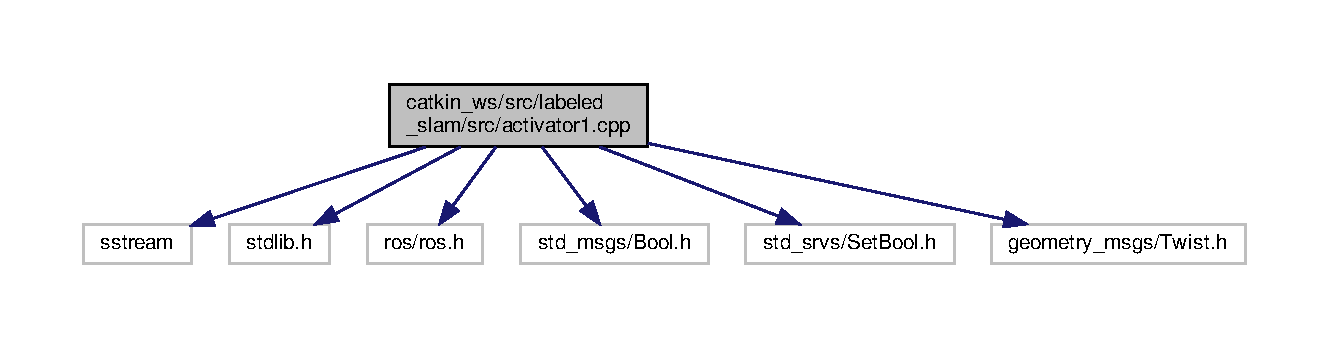
\includegraphics[width=350pt]{activator1_8cpp__incl}
\end{center}
\end{figure}
\subsection*{Functions}
\begin{DoxyCompactItemize}
\item 
void \hyperlink{activator1_8cpp_a27ad8e26c626eefcdbb0d7ee54a71896}{velocity\+\_\+callback} (const geometry\+\_\+msgs\+::\+Twist\+::\+Const\+Ptr \&received\+\_\+velocity)
\item 
bool \hyperlink{activator1_8cpp_a0e0b3479775a039d6aa169f4a86f4c5b}{path\+\_\+following\+\_\+activate} (std\+\_\+srvs\+::\+Set\+Bool\+::\+Request \&req, std\+\_\+srvs\+::\+Set\+Bool\+::\+Response \&response)
\item 
int \hyperlink{activator1_8cpp_a3c04138a5bfe5d72780bb7e82a18e627}{main} (int argc, char $\ast$$\ast$argv)
\end{DoxyCompactItemize}
\subsection*{Variables}
\begin{DoxyCompactItemize}
\item 
geometry\+\_\+msgs\+::\+Twist \hyperlink{activator1_8cpp_ad9ace2e48e2ae1119c2d4d0ae2ea25b8}{velocity\+\_\+to\+\_\+publish}
\item 
geometry\+\_\+msgs\+::\+Twist \hyperlink{activator1_8cpp_a17196b1618faaf44fb0a78bb5099d4ac}{zero\+\_\+velocity}
\item 
bool \hyperlink{activator1_8cpp_aa7bf910a844377996aa460aa46bcd5cc}{activation} = false
\end{DoxyCompactItemize}


\subsection{Function Documentation}
\mbox{\Hypertarget{activator1_8cpp_a3c04138a5bfe5d72780bb7e82a18e627}\label{activator1_8cpp_a3c04138a5bfe5d72780bb7e82a18e627}} 
\index{activator1.\+cpp@{activator1.\+cpp}!main@{main}}
\index{main@{main}!activator1.\+cpp@{activator1.\+cpp}}
\subsubsection{\texorpdfstring{main()}{main()}}
{\footnotesize\ttfamily int main (\begin{DoxyParamCaption}\item[{int}]{argc,  }\item[{char $\ast$$\ast$}]{argv }\end{DoxyParamCaption})}



Definition at line 20 of file activator1.\+cpp.

\mbox{\Hypertarget{activator1_8cpp_a0e0b3479775a039d6aa169f4a86f4c5b}\label{activator1_8cpp_a0e0b3479775a039d6aa169f4a86f4c5b}} 
\index{activator1.\+cpp@{activator1.\+cpp}!path\+\_\+following\+\_\+activate@{path\+\_\+following\+\_\+activate}}
\index{path\+\_\+following\+\_\+activate@{path\+\_\+following\+\_\+activate}!activator1.\+cpp@{activator1.\+cpp}}
\subsubsection{\texorpdfstring{path\+\_\+following\+\_\+activate()}{path\_following\_activate()}}
{\footnotesize\ttfamily bool path\+\_\+following\+\_\+activate (\begin{DoxyParamCaption}\item[{std\+\_\+srvs\+::\+Set\+Bool\+::\+Request \&}]{req,  }\item[{std\+\_\+srvs\+::\+Set\+Bool\+::\+Response \&}]{response }\end{DoxyParamCaption})}



Definition at line 67 of file activator1.\+cpp.

\mbox{\Hypertarget{activator1_8cpp_a27ad8e26c626eefcdbb0d7ee54a71896}\label{activator1_8cpp_a27ad8e26c626eefcdbb0d7ee54a71896}} 
\index{activator1.\+cpp@{activator1.\+cpp}!velocity\+\_\+callback@{velocity\+\_\+callback}}
\index{velocity\+\_\+callback@{velocity\+\_\+callback}!activator1.\+cpp@{activator1.\+cpp}}
\subsubsection{\texorpdfstring{velocity\+\_\+callback()}{velocity\_callback()}}
{\footnotesize\ttfamily void velocity\+\_\+callback (\begin{DoxyParamCaption}\item[{const geometry\+\_\+msgs\+::\+Twist\+::\+Const\+Ptr \&}]{received\+\_\+velocity }\end{DoxyParamCaption})}



Definition at line 81 of file activator1.\+cpp.



\subsection{Variable Documentation}
\mbox{\Hypertarget{activator1_8cpp_aa7bf910a844377996aa460aa46bcd5cc}\label{activator1_8cpp_aa7bf910a844377996aa460aa46bcd5cc}} 
\index{activator1.\+cpp@{activator1.\+cpp}!activation@{activation}}
\index{activation@{activation}!activator1.\+cpp@{activator1.\+cpp}}
\subsubsection{\texorpdfstring{activation}{activation}}
{\footnotesize\ttfamily bool activation = false}



Definition at line 14 of file activator1.\+cpp.

\mbox{\Hypertarget{activator1_8cpp_ad9ace2e48e2ae1119c2d4d0ae2ea25b8}\label{activator1_8cpp_ad9ace2e48e2ae1119c2d4d0ae2ea25b8}} 
\index{activator1.\+cpp@{activator1.\+cpp}!velocity\+\_\+to\+\_\+publish@{velocity\+\_\+to\+\_\+publish}}
\index{velocity\+\_\+to\+\_\+publish@{velocity\+\_\+to\+\_\+publish}!activator1.\+cpp@{activator1.\+cpp}}
\subsubsection{\texorpdfstring{velocity\+\_\+to\+\_\+publish}{velocity\_to\_publish}}
{\footnotesize\ttfamily geometry\+\_\+msgs\+::\+Twist velocity\+\_\+to\+\_\+publish}



Definition at line 11 of file activator1.\+cpp.

\mbox{\Hypertarget{activator1_8cpp_a17196b1618faaf44fb0a78bb5099d4ac}\label{activator1_8cpp_a17196b1618faaf44fb0a78bb5099d4ac}} 
\index{activator1.\+cpp@{activator1.\+cpp}!zero\+\_\+velocity@{zero\+\_\+velocity}}
\index{zero\+\_\+velocity@{zero\+\_\+velocity}!activator1.\+cpp@{activator1.\+cpp}}
\subsubsection{\texorpdfstring{zero\+\_\+velocity}{zero\_velocity}}
{\footnotesize\ttfamily geometry\+\_\+msgs\+::\+Twist zero\+\_\+velocity}



Definition at line 12 of file activator1.\+cpp.


\hypertarget{activator2_8cpp}{}\section{catkin\+\_\+ws/src/labeled\+\_\+slam/src/activator2.cpp File Reference}
\label{activator2_8cpp}\index{catkin\+\_\+ws/src/labeled\+\_\+slam/src/activator2.\+cpp@{catkin\+\_\+ws/src/labeled\+\_\+slam/src/activator2.\+cpp}}
{\ttfamily \#include $<$sstream$>$}\newline
{\ttfamily \#include $<$stdlib.\+h$>$}\newline
{\ttfamily \#include \char`\"{}ros/ros.\+h\char`\"{}}\newline
{\ttfamily \#include \char`\"{}std\+\_\+msgs/\+Bool.\+h\char`\"{}}\newline
{\ttfamily \#include \char`\"{}std\+\_\+srvs/\+Set\+Bool.\+h\char`\"{}}\newline
{\ttfamily \#include \char`\"{}geometry\+\_\+msgs/\+Twist.\+h\char`\"{}}\newline
Include dependency graph for activator2.\+cpp\+:\nopagebreak
\begin{figure}[H]
\begin{center}
\leavevmode
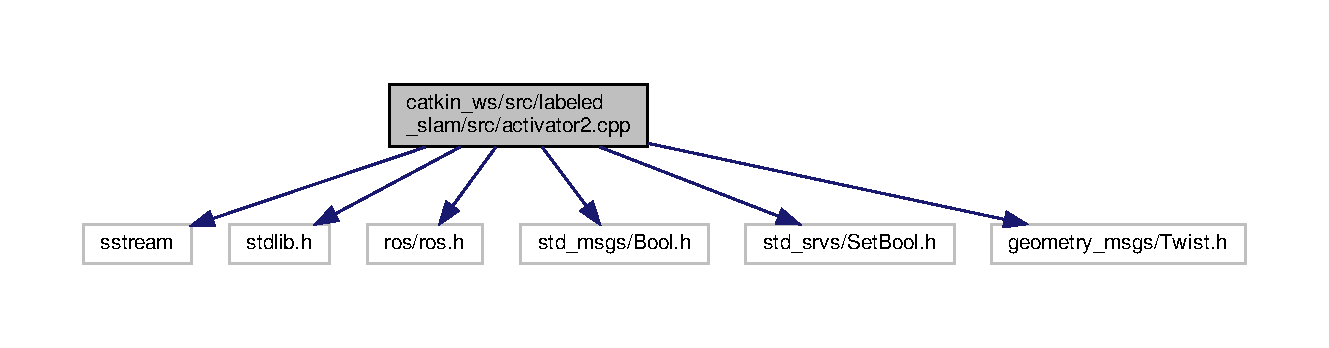
\includegraphics[width=350pt]{activator2_8cpp__incl}
\end{center}
\end{figure}
\subsection*{Functions}
\begin{DoxyCompactItemize}
\item 
void \hyperlink{activator2_8cpp_a27ad8e26c626eefcdbb0d7ee54a71896}{velocity\+\_\+callback} (const geometry\+\_\+msgs\+::\+Twist\+::\+Const\+Ptr \&received\+\_\+velocity)
\item 
bool \hyperlink{activator2_8cpp_a33c5721acde6590d4fdaf1c9324bf5fb}{driving\+\_\+activate} (std\+\_\+srvs\+::\+Set\+Bool\+::\+Request \&req, std\+\_\+srvs\+::\+Set\+Bool\+::\+Response \&response)
\item 
int \hyperlink{activator2_8cpp_a3c04138a5bfe5d72780bb7e82a18e627}{main} (int argc, char $\ast$$\ast$argv)
\end{DoxyCompactItemize}
\subsection*{Variables}
\begin{DoxyCompactItemize}
\item 
geometry\+\_\+msgs\+::\+Twist \hyperlink{activator2_8cpp_ad9ace2e48e2ae1119c2d4d0ae2ea25b8}{velocity\+\_\+to\+\_\+publish}
\item 
geometry\+\_\+msgs\+::\+Twist \hyperlink{activator2_8cpp_a17196b1618faaf44fb0a78bb5099d4ac}{zero\+\_\+velocity}
\item 
bool \hyperlink{activator2_8cpp_aa7bf910a844377996aa460aa46bcd5cc}{activation} = false
\end{DoxyCompactItemize}


\subsection{Function Documentation}
\mbox{\Hypertarget{activator2_8cpp_a33c5721acde6590d4fdaf1c9324bf5fb}\label{activator2_8cpp_a33c5721acde6590d4fdaf1c9324bf5fb}} 
\index{activator2.\+cpp@{activator2.\+cpp}!driving\+\_\+activate@{driving\+\_\+activate}}
\index{driving\+\_\+activate@{driving\+\_\+activate}!activator2.\+cpp@{activator2.\+cpp}}
\subsubsection{\texorpdfstring{driving\+\_\+activate()}{driving\_activate()}}
{\footnotesize\ttfamily bool driving\+\_\+activate (\begin{DoxyParamCaption}\item[{std\+\_\+srvs\+::\+Set\+Bool\+::\+Request \&}]{req,  }\item[{std\+\_\+srvs\+::\+Set\+Bool\+::\+Response \&}]{response }\end{DoxyParamCaption})}



Definition at line 65 of file activator2.\+cpp.

\mbox{\Hypertarget{activator2_8cpp_a3c04138a5bfe5d72780bb7e82a18e627}\label{activator2_8cpp_a3c04138a5bfe5d72780bb7e82a18e627}} 
\index{activator2.\+cpp@{activator2.\+cpp}!main@{main}}
\index{main@{main}!activator2.\+cpp@{activator2.\+cpp}}
\subsubsection{\texorpdfstring{main()}{main()}}
{\footnotesize\ttfamily int main (\begin{DoxyParamCaption}\item[{int}]{argc,  }\item[{char $\ast$$\ast$}]{argv }\end{DoxyParamCaption})}



Definition at line 20 of file activator2.\+cpp.

\mbox{\Hypertarget{activator2_8cpp_a27ad8e26c626eefcdbb0d7ee54a71896}\label{activator2_8cpp_a27ad8e26c626eefcdbb0d7ee54a71896}} 
\index{activator2.\+cpp@{activator2.\+cpp}!velocity\+\_\+callback@{velocity\+\_\+callback}}
\index{velocity\+\_\+callback@{velocity\+\_\+callback}!activator2.\+cpp@{activator2.\+cpp}}
\subsubsection{\texorpdfstring{velocity\+\_\+callback()}{velocity\_callback()}}
{\footnotesize\ttfamily void velocity\+\_\+callback (\begin{DoxyParamCaption}\item[{const geometry\+\_\+msgs\+::\+Twist\+::\+Const\+Ptr \&}]{received\+\_\+velocity }\end{DoxyParamCaption})}



Definition at line 80 of file activator2.\+cpp.



\subsection{Variable Documentation}
\mbox{\Hypertarget{activator2_8cpp_aa7bf910a844377996aa460aa46bcd5cc}\label{activator2_8cpp_aa7bf910a844377996aa460aa46bcd5cc}} 
\index{activator2.\+cpp@{activator2.\+cpp}!activation@{activation}}
\index{activation@{activation}!activator2.\+cpp@{activator2.\+cpp}}
\subsubsection{\texorpdfstring{activation}{activation}}
{\footnotesize\ttfamily bool activation = false}



Definition at line 14 of file activator2.\+cpp.

\mbox{\Hypertarget{activator2_8cpp_ad9ace2e48e2ae1119c2d4d0ae2ea25b8}\label{activator2_8cpp_ad9ace2e48e2ae1119c2d4d0ae2ea25b8}} 
\index{activator2.\+cpp@{activator2.\+cpp}!velocity\+\_\+to\+\_\+publish@{velocity\+\_\+to\+\_\+publish}}
\index{velocity\+\_\+to\+\_\+publish@{velocity\+\_\+to\+\_\+publish}!activator2.\+cpp@{activator2.\+cpp}}
\subsubsection{\texorpdfstring{velocity\+\_\+to\+\_\+publish}{velocity\_to\_publish}}
{\footnotesize\ttfamily geometry\+\_\+msgs\+::\+Twist velocity\+\_\+to\+\_\+publish}



Definition at line 11 of file activator2.\+cpp.

\mbox{\Hypertarget{activator2_8cpp_a17196b1618faaf44fb0a78bb5099d4ac}\label{activator2_8cpp_a17196b1618faaf44fb0a78bb5099d4ac}} 
\index{activator2.\+cpp@{activator2.\+cpp}!zero\+\_\+velocity@{zero\+\_\+velocity}}
\index{zero\+\_\+velocity@{zero\+\_\+velocity}!activator2.\+cpp@{activator2.\+cpp}}
\subsubsection{\texorpdfstring{zero\+\_\+velocity}{zero\_velocity}}
{\footnotesize\ttfamily geometry\+\_\+msgs\+::\+Twist zero\+\_\+velocity}



Definition at line 12 of file activator2.\+cpp.


\hypertarget{command__recognition_8py}{}\section{catkin\+\_\+ws/src/labeled\+\_\+slam/src/command\+\_\+recognition.py File Reference}
\label{command__recognition_8py}\index{catkin\+\_\+ws/src/labeled\+\_\+slam/src/command\+\_\+recognition.\+py@{catkin\+\_\+ws/src/labeled\+\_\+slam/src/command\+\_\+recognition.\+py}}
\subsection*{Classes}
\begin{DoxyCompactItemize}
\item 
class \hyperlink{classcommand__recognition_1_1_main___speech___controller}{command\+\_\+recognition.\+Main\+\_\+\+Speech\+\_\+\+Controller}
\begin{DoxyCompactList}\small\item\em Mother class. \end{DoxyCompactList}\end{DoxyCompactItemize}
\subsection*{Namespaces}
\begin{DoxyCompactItemize}
\item 
 \hyperlink{namespacecommand__recognition}{command\+\_\+recognition}
\end{DoxyCompactItemize}
\subsection*{Functions}
\begin{DoxyCompactItemize}
\item 
def \hyperlink{namespacecommand__recognition_a7ea48f781ea104f0a02f0b755f671b52}{command\+\_\+recognition.\+main} ()
\begin{DoxyCompactList}\small\item\em Main, initializes the class and starts the node. \end{DoxyCompactList}\end{DoxyCompactItemize}

\hypertarget{logic__node_8cpp}{}\section{catkin\+\_\+ws/src/labeled\+\_\+slam/src/logic\+\_\+node.cpp File Reference}
\label{logic__node_8cpp}\index{catkin\+\_\+ws/src/labeled\+\_\+slam/src/logic\+\_\+node.\+cpp@{catkin\+\_\+ws/src/labeled\+\_\+slam/src/logic\+\_\+node.\+cpp}}
{\ttfamily \#include \char`\"{}State\+Machine.\+h\char`\"{}}\newline
{\ttfamily \#include \char`\"{}ros/ros.\+h\char`\"{}}\newline
Include dependency graph for logic\+\_\+node.\+cpp\+:\nopagebreak
\begin{figure}[H]
\begin{center}
\leavevmode
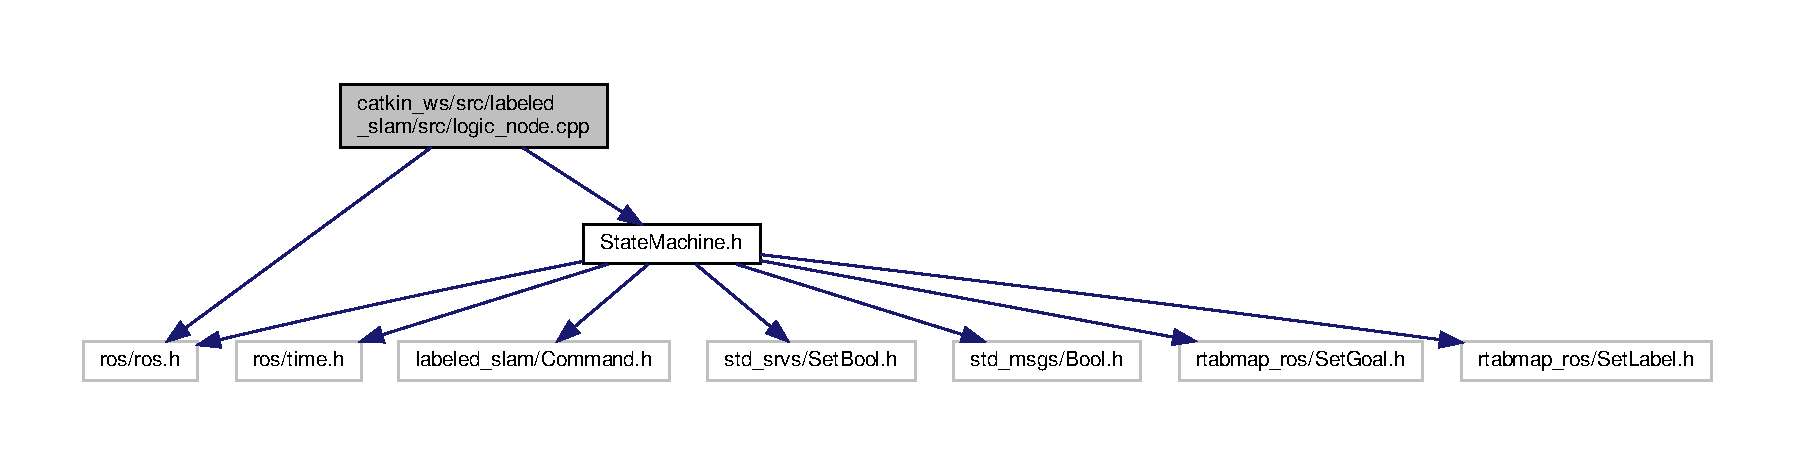
\includegraphics[width=350pt]{logic__node_8cpp__incl}
\end{center}
\end{figure}
\subsection*{Functions}
\begin{DoxyCompactItemize}
\item 
int \hyperlink{logic__node_8cpp_a3c04138a5bfe5d72780bb7e82a18e627}{main} (int argc, char $\ast$$\ast$argv)
\begin{DoxyCompactList}\small\item\em This node implements the main logic of the labeled\+\_\+slam project. \end{DoxyCompactList}\end{DoxyCompactItemize}


\subsection{Function Documentation}
\mbox{\Hypertarget{logic__node_8cpp_a3c04138a5bfe5d72780bb7e82a18e627}\label{logic__node_8cpp_a3c04138a5bfe5d72780bb7e82a18e627}} 
\index{logic\+\_\+node.\+cpp@{logic\+\_\+node.\+cpp}!main@{main}}
\index{main@{main}!logic\+\_\+node.\+cpp@{logic\+\_\+node.\+cpp}}
\subsubsection{\texorpdfstring{main()}{main()}}
{\footnotesize\ttfamily int main (\begin{DoxyParamCaption}\item[{int}]{argc,  }\item[{char $\ast$$\ast$}]{argv }\end{DoxyParamCaption})}



This node implements the main logic of the labeled\+\_\+slam project. 

The core object of this node is state\+\_\+machine The c++ \char`\"{}state\char`\"{}-\/pattern is used to imlement the state machine in an object-\/ oriented, safe and maintainable way Possible states of the state machine are \char`\"{}\+D\+R\+I\+V\+I\+N\+G\char`\"{}, \char`\"{}\+L\+I\+S\+T\+E\+N\+I\+N\+G\char`\"{} and \char`\"{}\+G\+O\+\_\+\+T\+O\char`\"{} 

Definition at line 12 of file logic\+\_\+node.\+cpp.


\hypertarget{path__follower_8cpp}{}\section{catkin\+\_\+ws/src/labeled\+\_\+slam/src/path\+\_\+follower.cpp File Reference}
\label{path__follower_8cpp}\index{catkin\+\_\+ws/src/labeled\+\_\+slam/src/path\+\_\+follower.\+cpp@{catkin\+\_\+ws/src/labeled\+\_\+slam/src/path\+\_\+follower.\+cpp}}
{\ttfamily \#include $<$sstream$>$}\newline
{\ttfamily \#include $<$stdlib.\+h$>$}\newline
{\ttfamily \#include \char`\"{}ros/ros.\+h\char`\"{}}\newline
{\ttfamily \#include \char`\"{}std\+\_\+msgs/\+Header.\+h\char`\"{}}\newline
{\ttfamily \#include \char`\"{}geometry\+\_\+msgs/\+Point.\+h\char`\"{}}\newline
{\ttfamily \#include \char`\"{}geometry\+\_\+msgs/\+Pose.\+h\char`\"{}}\newline
{\ttfamily \#include \char`\"{}geometry\+\_\+msgs/\+Twist.\+h\char`\"{}}\newline
{\ttfamily \#include \char`\"{}geometry\+\_\+msgs/\+Vector3.\+h\char`\"{}}\newline
{\ttfamily \#include \char`\"{}geometry\+\_\+msgs/\+Transform\+Stamped.\+h\char`\"{}}\newline
{\ttfamily \#include \char`\"{}geometry\+\_\+msgs/\+Transform.\+h\char`\"{}}\newline
{\ttfamily \#include $<$tf/transform\+\_\+listener.\+h$>$}\newline
{\ttfamily \#include \char`\"{}nav\+\_\+msgs/\+Path.\+h\char`\"{}}\newline
{\ttfamily \#include \char`\"{}tf/\+Linear\+Math/\+Transform.\+h\char`\"{}}\newline
{\ttfamily \#include \char`\"{}tf/\+Linear\+Math/\+Matrix3x3.\+h\char`\"{}}\newline
{\ttfamily \#include $<$string$>$}\newline
{\ttfamily \#include $<$array$>$}\newline
{\ttfamily \#include $<$cmath$>$}\newline
Include dependency graph for path\+\_\+follower.\+cpp\+:\nopagebreak
\begin{figure}[H]
\begin{center}
\leavevmode
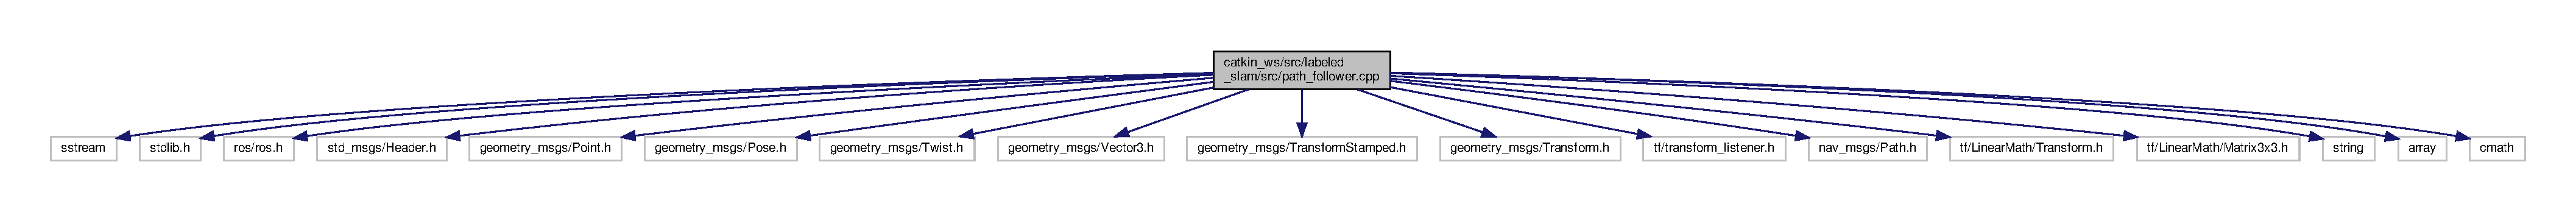
\includegraphics[width=350pt]{path__follower_8cpp__incl}
\end{center}
\end{figure}
\subsection*{Functions}
\begin{DoxyCompactItemize}
\item 
void \hyperlink{path__follower_8cpp_aa9a42b10b0895a8dea5f7a3e53622445}{path\+\_\+callback} (const nav\+\_\+msgs\+::\+Path\+::\+Const\+Ptr \&received\+\_\+path)
\item 
bool \hyperlink{path__follower_8cpp_a6580d4219bb711f9f65ecdc5ae43a7b4}{proximity\+\_\+check} (geometry\+\_\+msgs\+::\+Point goal, tf\+::\+Point current)
\item 
bool \hyperlink{path__follower_8cpp_a381fc6065d560c219bdf0733ccd3ba13}{angle\+\_\+check} (float goal\+\_\+angle, tf\+Scalar yaw)
\item 
int \hyperlink{path__follower_8cpp_a3c04138a5bfe5d72780bb7e82a18e627}{main} (int argc, char $\ast$$\ast$argv)
\end{DoxyCompactItemize}
\subsection*{Variables}
\begin{DoxyCompactItemize}
\item 
std\+::vector$<$ geometry\+\_\+msgs\+::\+Pose\+Stamped $>$ \hyperlink{path__follower_8cpp_a06bc50440cb7aad0ef28a930499574c5}{current\+\_\+path}
\item 
std\+::vector$<$ geometry\+\_\+msgs\+::\+Pose\+Stamped $>$\+::iterator \hyperlink{path__follower_8cpp_afd300c5785c540c1370de4c45066f345}{it}
\item 
geometry\+\_\+msgs\+::\+Point \hyperlink{path__follower_8cpp_a1dd788339a5b3696b0f6273eda3136fc}{goal\+\_\+position}
\begin{DoxyCompactList}\small\item\em Goal position on map. \end{DoxyCompactList}\item 
geometry\+\_\+msgs\+::\+Quaternion \hyperlink{path__follower_8cpp_afbef336bbcb2c1100f1e01e10a7beee6}{goal\+\_\+orientation}
\begin{DoxyCompactList}\small\item\em Goal orientation on map. \end{DoxyCompactList}\item 
geometry\+\_\+msgs\+::\+Twist \hyperlink{path__follower_8cpp_ad9ace2e48e2ae1119c2d4d0ae2ea25b8}{velocity\+\_\+to\+\_\+publish}
\begin{DoxyCompactList}\small\item\em Velocity sent to robot driver. \end{DoxyCompactList}\item 
float \hyperlink{path__follower_8cpp_a12fa92d7da4d3dad3d9962e706c7eb60}{tolerance\+\_\+angle}
\item 
float \hyperlink{path__follower_8cpp_a7e58fbe5f78a53ae55c2fc5ff2e690d0}{tolerance\+\_\+dist}
\end{DoxyCompactItemize}


\subsection{Function Documentation}
\mbox{\Hypertarget{path__follower_8cpp_a381fc6065d560c219bdf0733ccd3ba13}\label{path__follower_8cpp_a381fc6065d560c219bdf0733ccd3ba13}} 
\index{path\+\_\+follower.\+cpp@{path\+\_\+follower.\+cpp}!angle\+\_\+check@{angle\+\_\+check}}
\index{angle\+\_\+check@{angle\+\_\+check}!path\+\_\+follower.\+cpp@{path\+\_\+follower.\+cpp}}
\subsubsection{\texorpdfstring{angle\+\_\+check()}{angle\_check()}}
{\footnotesize\ttfamily bool angle\+\_\+check (\begin{DoxyParamCaption}\item[{float}]{goal\+\_\+angle,  }\item[{tf\+Scalar}]{yaw }\end{DoxyParamCaption})}



Definition at line 213 of file path\+\_\+follower.\+cpp.

\mbox{\Hypertarget{path__follower_8cpp_a3c04138a5bfe5d72780bb7e82a18e627}\label{path__follower_8cpp_a3c04138a5bfe5d72780bb7e82a18e627}} 
\index{path\+\_\+follower.\+cpp@{path\+\_\+follower.\+cpp}!main@{main}}
\index{main@{main}!path\+\_\+follower.\+cpp@{path\+\_\+follower.\+cpp}}
\subsubsection{\texorpdfstring{main()}{main()}}
{\footnotesize\ttfamily int main (\begin{DoxyParamCaption}\item[{int}]{argc,  }\item[{char $\ast$$\ast$}]{argv }\end{DoxyParamCaption})}

The node subscribes to a TF topic, and gets the current position of the robot as a base\+\_\+link. It receives from the callback the goal position, and publishes the required position as a geometry\+\_\+msgs\+::\+Twist to reach that position. The path follower computes the angle difference between the goal position and the robot orientation. The robot then rotates left or right accordingly, until it is on the same line as the goal orientation. At that moment, the robot moves forward. All \char`\"{}robot movements\char`\"{} are considered as published veolcities as geometry\+\_\+msgs\+::\+Twist messages. Current position of robot

Current orientation of robot in quaternion 

Definition at line 50 of file path\+\_\+follower.\+cpp.

\mbox{\Hypertarget{path__follower_8cpp_aa9a42b10b0895a8dea5f7a3e53622445}\label{path__follower_8cpp_aa9a42b10b0895a8dea5f7a3e53622445}} 
\index{path\+\_\+follower.\+cpp@{path\+\_\+follower.\+cpp}!path\+\_\+callback@{path\+\_\+callback}}
\index{path\+\_\+callback@{path\+\_\+callback}!path\+\_\+follower.\+cpp@{path\+\_\+follower.\+cpp}}
\subsubsection{\texorpdfstring{path\+\_\+callback()}{path\_callback()}}
{\footnotesize\ttfamily void path\+\_\+callback (\begin{DoxyParamCaption}\item[{const nav\+\_\+msgs\+::\+Path\+::\+Const\+Ptr \&}]{received\+\_\+path }\end{DoxyParamCaption})}

Path Callback Callback function for the path follower. The node subscribes to the nav\+\_\+msgs\+::\+Path published by rtabmap. These messages provide the node with the goal position and orientation to be achived when in G\+O\+\_\+\+T\+O\+\_\+\+G\+O\+AL M\+O\+DE. The callback is used to initialize the two gobal variables goal\+\_\+position and goal\+\_\+orientation used in the 

Definition at line 188 of file path\+\_\+follower.\+cpp.

\mbox{\Hypertarget{path__follower_8cpp_a6580d4219bb711f9f65ecdc5ae43a7b4}\label{path__follower_8cpp_a6580d4219bb711f9f65ecdc5ae43a7b4}} 
\index{path\+\_\+follower.\+cpp@{path\+\_\+follower.\+cpp}!proximity\+\_\+check@{proximity\+\_\+check}}
\index{proximity\+\_\+check@{proximity\+\_\+check}!path\+\_\+follower.\+cpp@{path\+\_\+follower.\+cpp}}
\subsubsection{\texorpdfstring{proximity\+\_\+check()}{proximity\_check()}}
{\footnotesize\ttfamily bool proximity\+\_\+check (\begin{DoxyParamCaption}\item[{geometry\+\_\+msgs\+::\+Point}]{goal,  }\item[{tf\+::\+Point}]{current }\end{DoxyParamCaption})}

Proximity Check The function checks whether the robot is close enough to the target position and returns a bool. It takes as input and uses the xy coordinates of the goal position and current positions. If the robot is close enough, it returns a true, otherwise returns a false. 

Definition at line 205 of file path\+\_\+follower.\+cpp.



\subsection{Variable Documentation}
\mbox{\Hypertarget{path__follower_8cpp_a06bc50440cb7aad0ef28a930499574c5}\label{path__follower_8cpp_a06bc50440cb7aad0ef28a930499574c5}} 
\index{path\+\_\+follower.\+cpp@{path\+\_\+follower.\+cpp}!current\+\_\+path@{current\+\_\+path}}
\index{current\+\_\+path@{current\+\_\+path}!path\+\_\+follower.\+cpp@{path\+\_\+follower.\+cpp}}
\subsubsection{\texorpdfstring{current\+\_\+path}{current\_path}}
{\footnotesize\ttfamily std\+::vector$<$geometry\+\_\+msgs\+::\+Pose\+Stamped$>$ current\+\_\+path}



Definition at line 31 of file path\+\_\+follower.\+cpp.

\mbox{\Hypertarget{path__follower_8cpp_afbef336bbcb2c1100f1e01e10a7beee6}\label{path__follower_8cpp_afbef336bbcb2c1100f1e01e10a7beee6}} 
\index{path\+\_\+follower.\+cpp@{path\+\_\+follower.\+cpp}!goal\+\_\+orientation@{goal\+\_\+orientation}}
\index{goal\+\_\+orientation@{goal\+\_\+orientation}!path\+\_\+follower.\+cpp@{path\+\_\+follower.\+cpp}}
\subsubsection{\texorpdfstring{goal\+\_\+orientation}{goal\_orientation}}
{\footnotesize\ttfamily geometry\+\_\+msgs\+::\+Quaternion goal\+\_\+orientation}



Goal orientation on map. 



Definition at line 36 of file path\+\_\+follower.\+cpp.

\mbox{\Hypertarget{path__follower_8cpp_a1dd788339a5b3696b0f6273eda3136fc}\label{path__follower_8cpp_a1dd788339a5b3696b0f6273eda3136fc}} 
\index{path\+\_\+follower.\+cpp@{path\+\_\+follower.\+cpp}!goal\+\_\+position@{goal\+\_\+position}}
\index{goal\+\_\+position@{goal\+\_\+position}!path\+\_\+follower.\+cpp@{path\+\_\+follower.\+cpp}}
\subsubsection{\texorpdfstring{goal\+\_\+position}{goal\_position}}
{\footnotesize\ttfamily geometry\+\_\+msgs\+::\+Point goal\+\_\+position}



Goal position on map. 



Definition at line 34 of file path\+\_\+follower.\+cpp.

\mbox{\Hypertarget{path__follower_8cpp_afd300c5785c540c1370de4c45066f345}\label{path__follower_8cpp_afd300c5785c540c1370de4c45066f345}} 
\index{path\+\_\+follower.\+cpp@{path\+\_\+follower.\+cpp}!it@{it}}
\index{it@{it}!path\+\_\+follower.\+cpp@{path\+\_\+follower.\+cpp}}
\subsubsection{\texorpdfstring{it}{it}}
{\footnotesize\ttfamily std\+::vector$<$geometry\+\_\+msgs\+::\+Pose\+Stamped$>$\+::iterator it}



Definition at line 32 of file path\+\_\+follower.\+cpp.

\mbox{\Hypertarget{path__follower_8cpp_a12fa92d7da4d3dad3d9962e706c7eb60}\label{path__follower_8cpp_a12fa92d7da4d3dad3d9962e706c7eb60}} 
\index{path\+\_\+follower.\+cpp@{path\+\_\+follower.\+cpp}!tolerance\+\_\+angle@{tolerance\+\_\+angle}}
\index{tolerance\+\_\+angle@{tolerance\+\_\+angle}!path\+\_\+follower.\+cpp@{path\+\_\+follower.\+cpp}}
\subsubsection{\texorpdfstring{tolerance\+\_\+angle}{tolerance\_angle}}
{\footnotesize\ttfamily float tolerance\+\_\+angle}



Definition at line 40 of file path\+\_\+follower.\+cpp.

\mbox{\Hypertarget{path__follower_8cpp_a7e58fbe5f78a53ae55c2fc5ff2e690d0}\label{path__follower_8cpp_a7e58fbe5f78a53ae55c2fc5ff2e690d0}} 
\index{path\+\_\+follower.\+cpp@{path\+\_\+follower.\+cpp}!tolerance\+\_\+dist@{tolerance\+\_\+dist}}
\index{tolerance\+\_\+dist@{tolerance\+\_\+dist}!path\+\_\+follower.\+cpp@{path\+\_\+follower.\+cpp}}
\subsubsection{\texorpdfstring{tolerance\+\_\+dist}{tolerance\_dist}}
{\footnotesize\ttfamily float tolerance\+\_\+dist}



Definition at line 40 of file path\+\_\+follower.\+cpp.

\mbox{\Hypertarget{path__follower_8cpp_ad9ace2e48e2ae1119c2d4d0ae2ea25b8}\label{path__follower_8cpp_ad9ace2e48e2ae1119c2d4d0ae2ea25b8}} 
\index{path\+\_\+follower.\+cpp@{path\+\_\+follower.\+cpp}!velocity\+\_\+to\+\_\+publish@{velocity\+\_\+to\+\_\+publish}}
\index{velocity\+\_\+to\+\_\+publish@{velocity\+\_\+to\+\_\+publish}!path\+\_\+follower.\+cpp@{path\+\_\+follower.\+cpp}}
\subsubsection{\texorpdfstring{velocity\+\_\+to\+\_\+publish}{velocity\_to\_publish}}
{\footnotesize\ttfamily geometry\+\_\+msgs\+::\+Twist velocity\+\_\+to\+\_\+publish}



Velocity sent to robot driver. 



Definition at line 38 of file path\+\_\+follower.\+cpp.


\hypertarget{_state___d_r_i_v_i_n_g_8cpp}{}\section{catkin\+\_\+ws/src/labeled\+\_\+slam/src/\+State\+Machine/\+State\+\_\+\+D\+R\+I\+V\+I\+NG.cpp File Reference}
\label{_state___d_r_i_v_i_n_g_8cpp}\index{catkin\+\_\+ws/src/labeled\+\_\+slam/src/\+State\+Machine/\+State\+\_\+\+D\+R\+I\+V\+I\+N\+G.\+cpp@{catkin\+\_\+ws/src/labeled\+\_\+slam/src/\+State\+Machine/\+State\+\_\+\+D\+R\+I\+V\+I\+N\+G.\+cpp}}
{\ttfamily \#include \char`\"{}State\+\_\+\+D\+R\+I\+V\+I\+N\+G.\+h\char`\"{}}\newline
{\ttfamily \#include \char`\"{}State\+\_\+\+L\+I\+S\+T\+E\+N\+I\+N\+G.\+h\char`\"{}}\newline
{\ttfamily \#include \char`\"{}State\+Machine.\+h\char`\"{}}\newline
Include dependency graph for State\+\_\+\+D\+R\+I\+V\+I\+N\+G.\+cpp\+:\nopagebreak
\begin{figure}[H]
\begin{center}
\leavevmode
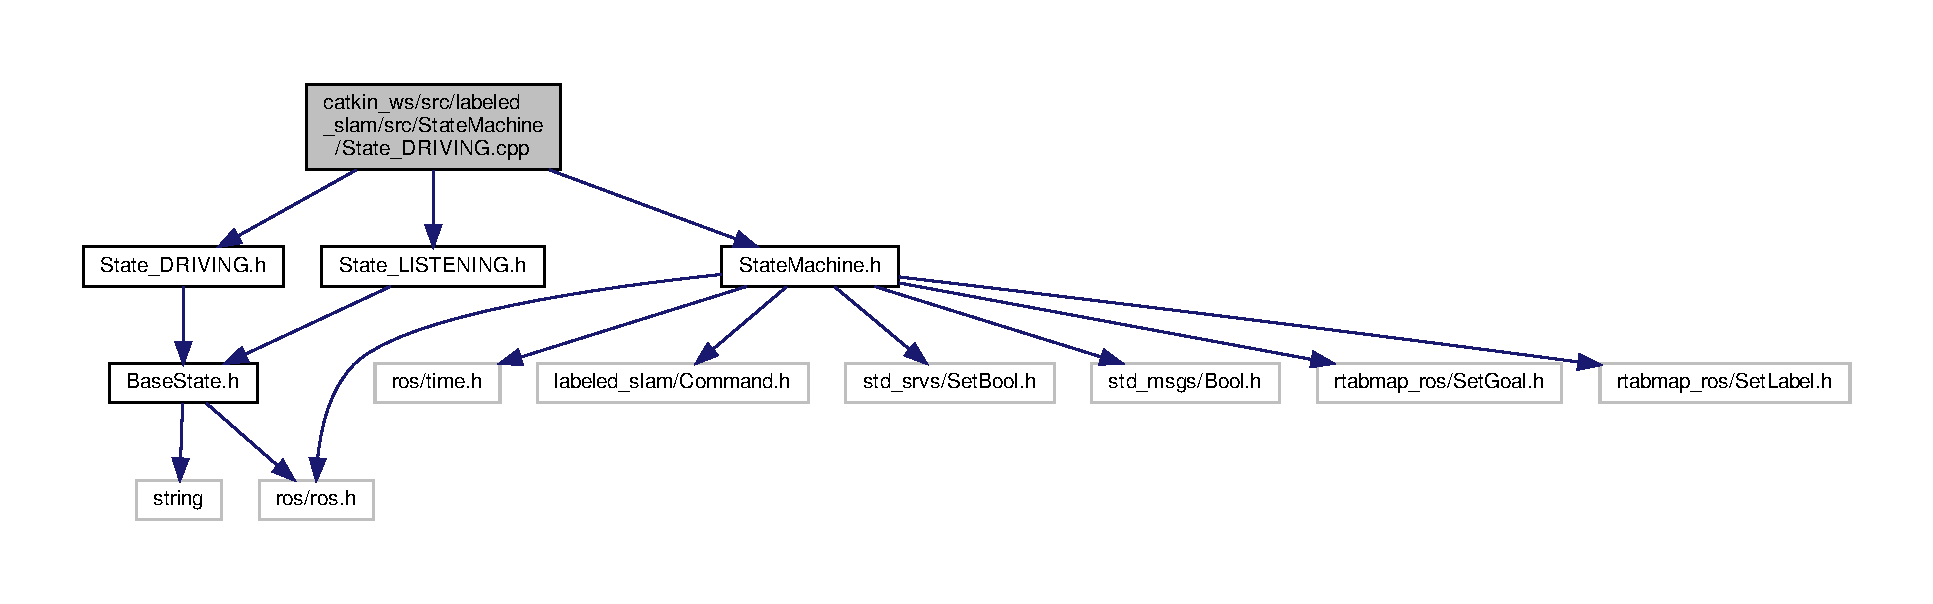
\includegraphics[width=350pt]{_state___d_r_i_v_i_n_g_8cpp__incl}
\end{center}
\end{figure}

\hypertarget{_state___g_o___t_o_8cpp}{}\section{catkin\+\_\+ws/src/labeled\+\_\+slam/src/\+State\+Machine/\+State\+\_\+\+G\+O\+\_\+\+TO.cpp File Reference}
\label{_state___g_o___t_o_8cpp}\index{catkin\+\_\+ws/src/labeled\+\_\+slam/src/\+State\+Machine/\+State\+\_\+\+G\+O\+\_\+\+T\+O.\+cpp@{catkin\+\_\+ws/src/labeled\+\_\+slam/src/\+State\+Machine/\+State\+\_\+\+G\+O\+\_\+\+T\+O.\+cpp}}
{\ttfamily \#include \char`\"{}State\+\_\+\+G\+O\+\_\+\+T\+O.\+h\char`\"{}}\newline
{\ttfamily \#include \char`\"{}State\+\_\+\+L\+I\+S\+T\+E\+N\+I\+N\+G.\+h\char`\"{}}\newline
{\ttfamily \#include \char`\"{}State\+Machine.\+h\char`\"{}}\newline
Include dependency graph for State\+\_\+\+G\+O\+\_\+\+T\+O.\+cpp\+:
\nopagebreak
\begin{figure}[H]
\begin{center}
\leavevmode
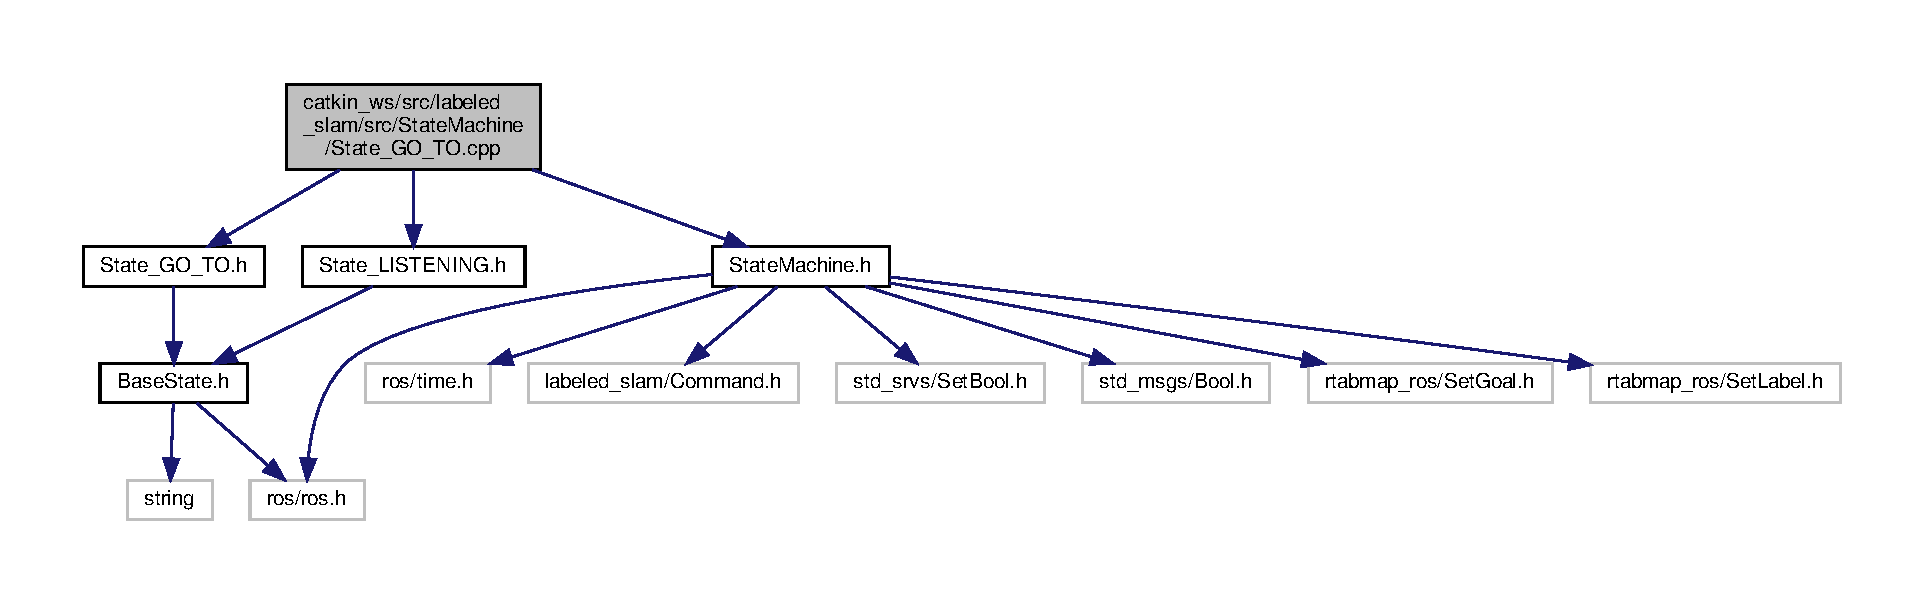
\includegraphics[width=350pt]{_state___g_o___t_o_8cpp__incl}
\end{center}
\end{figure}

\hypertarget{_state___l_i_s_t_e_n_i_n_g_8cpp}{}\section{catkin\+\_\+ws/src/labeled\+\_\+slam/src/\+State\+Machine/\+State\+\_\+\+L\+I\+S\+T\+E\+N\+I\+NG.cpp File Reference}
\label{_state___l_i_s_t_e_n_i_n_g_8cpp}\index{catkin\+\_\+ws/src/labeled\+\_\+slam/src/\+State\+Machine/\+State\+\_\+\+L\+I\+S\+T\+E\+N\+I\+N\+G.\+cpp@{catkin\+\_\+ws/src/labeled\+\_\+slam/src/\+State\+Machine/\+State\+\_\+\+L\+I\+S\+T\+E\+N\+I\+N\+G.\+cpp}}
{\ttfamily \#include \char`\"{}State\+\_\+\+L\+I\+S\+T\+E\+N\+I\+N\+G.\+h\char`\"{}}\newline
{\ttfamily \#include \char`\"{}State\+\_\+\+G\+O\+\_\+\+T\+O.\+h\char`\"{}}\newline
{\ttfamily \#include \char`\"{}State\+\_\+\+D\+R\+I\+V\+I\+N\+G.\+h\char`\"{}}\newline
{\ttfamily \#include \char`\"{}State\+Machine.\+h\char`\"{}}\newline
Include dependency graph for State\+\_\+\+L\+I\+S\+T\+E\+N\+I\+N\+G.\+cpp\+:\nopagebreak
\begin{figure}[H]
\begin{center}
\leavevmode
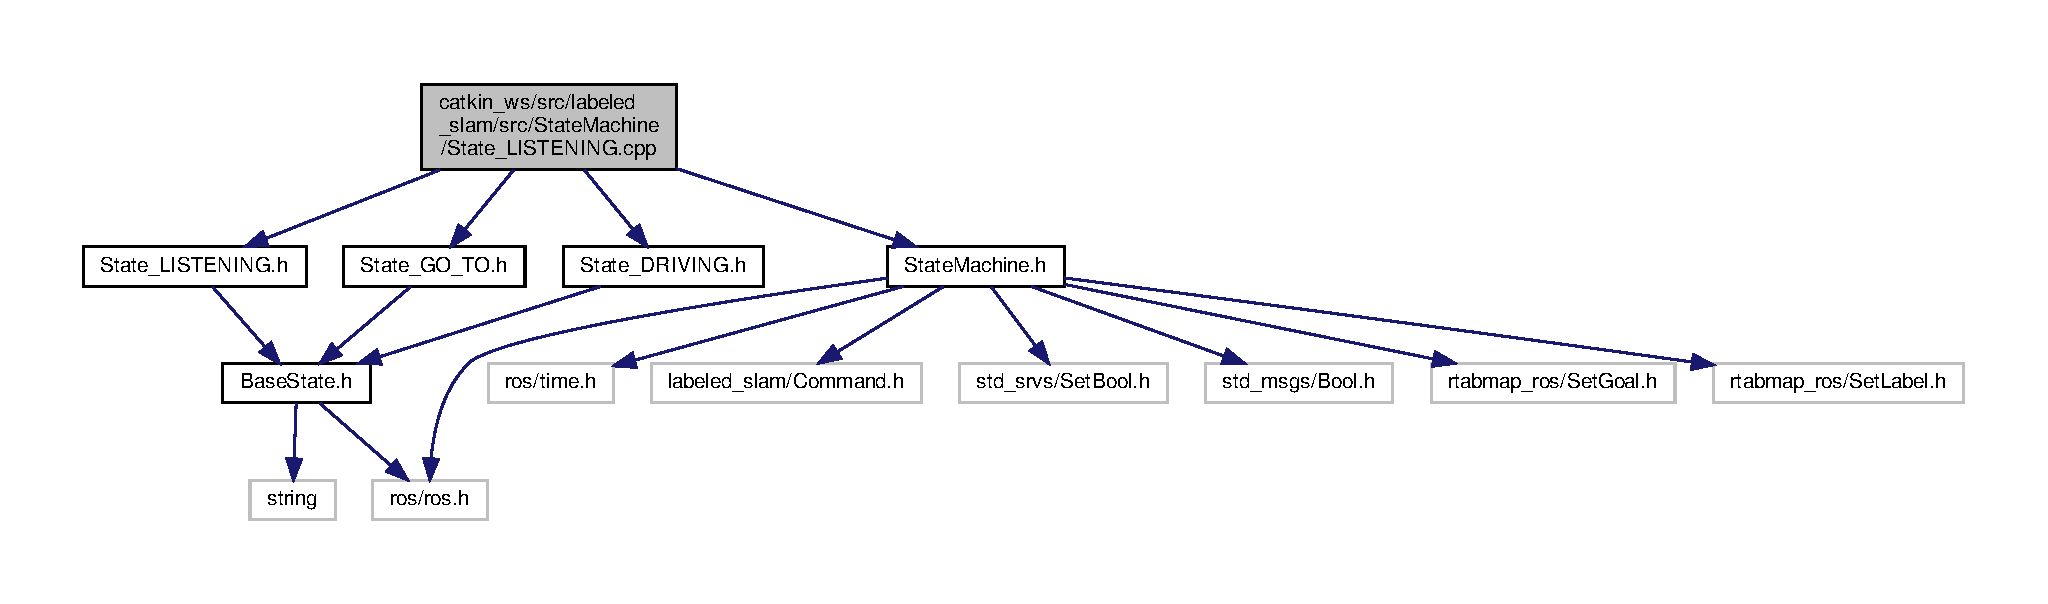
\includegraphics[width=350pt]{_state___l_i_s_t_e_n_i_n_g_8cpp__incl}
\end{center}
\end{figure}

\hypertarget{_state_machine_8cpp}{}\section{catkin\+\_\+ws/src/labeled\+\_\+slam/src/\+State\+Machine/\+State\+Machine.cpp File Reference}
\label{_state_machine_8cpp}\index{catkin\+\_\+ws/src/labeled\+\_\+slam/src/\+State\+Machine/\+State\+Machine.\+cpp@{catkin\+\_\+ws/src/labeled\+\_\+slam/src/\+State\+Machine/\+State\+Machine.\+cpp}}
{\ttfamily \#include \char`\"{}State\+Machine.\+h\char`\"{}}\newline
{\ttfamily \#include \char`\"{}State\+\_\+\+D\+R\+I\+V\+I\+N\+G.\+h\char`\"{}}\newline
{\ttfamily \#include \char`\"{}State\+\_\+\+G\+O\+\_\+\+T\+O.\+h\char`\"{}}\newline
{\ttfamily \#include \char`\"{}State\+\_\+\+L\+I\+S\+T\+E\+N\+I\+N\+G.\+h\char`\"{}}\newline
{\ttfamily \#include $<$iostream$>$}\newline
Include dependency graph for State\+Machine.\+cpp\+:\nopagebreak
\begin{figure}[H]
\begin{center}
\leavevmode
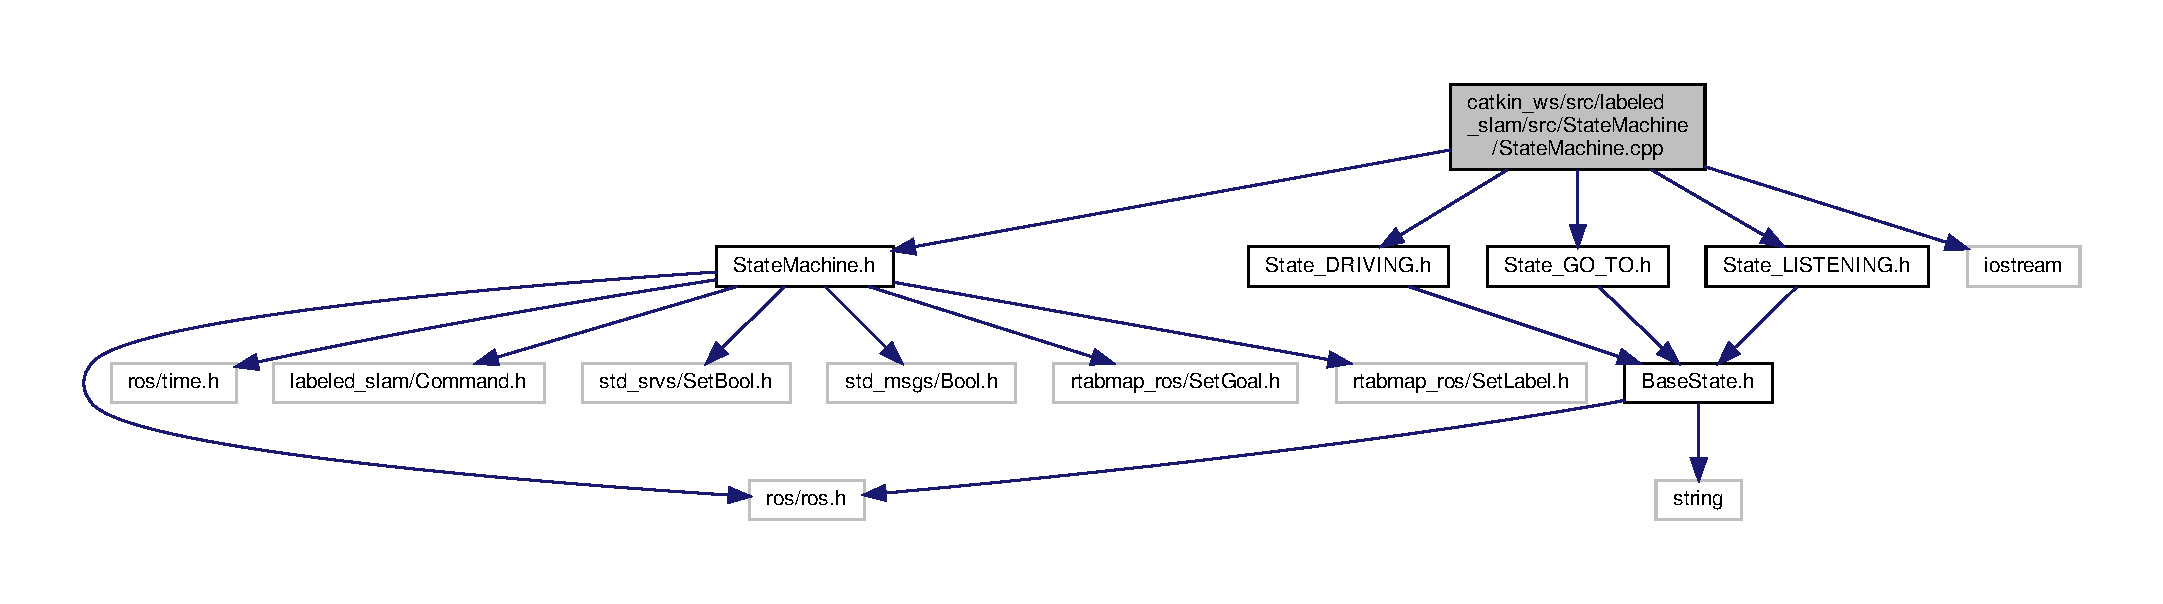
\includegraphics[width=350pt]{_state_machine_8cpp__incl}
\end{center}
\end{figure}

\hypertarget{velocity__forwarder_8cpp}{}\section{src/velocity\+\_\+forwarder.cpp File Reference}
\label{velocity__forwarder_8cpp}\index{src/velocity\+\_\+forwarder.\+cpp@{src/velocity\+\_\+forwarder.\+cpp}}
{\ttfamily \#include $<$ros/ros.\+h$>$}\\*
{\ttfamily \#include $<$geometry\+\_\+msgs/\+Twist.\+h$>$}\\*
{\ttfamily \#include \char`\"{}std\+\_\+msgs/\+String.\+h\char`\"{}}\\*
{\ttfamily \#include $<$sstream$>$}\\*
Include dependency graph for velocity\+\_\+forwarder.\+cpp\+:\nopagebreak
\begin{figure}[H]
\begin{center}
\leavevmode
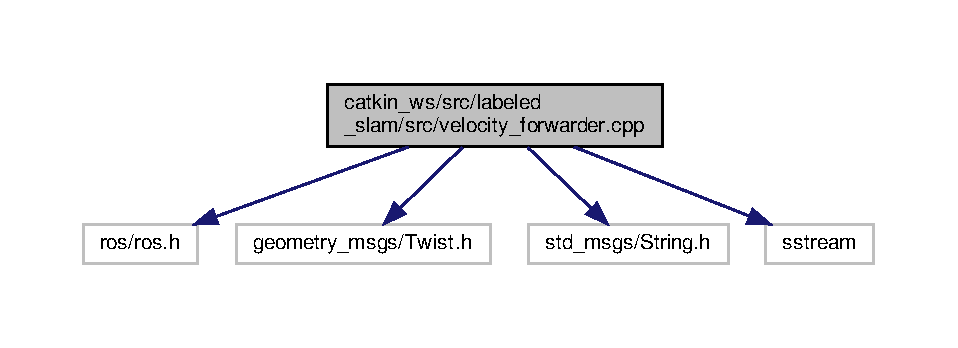
\includegraphics[width=350pt]{velocity__forwarder_8cpp__incl}
\end{center}
\end{figure}
\subsection*{Functions}
\begin{DoxyCompactItemize}
\item 
void \hyperlink{velocity__forwarder_8cpp_a5121f63bb791a335dbb5110dd1afbaa9}{Callback\+\_\+activator1} (const geometry\+\_\+msgs\+::\+Twist \&\hyperlink{velocity__forwarder_8cpp_aba2f97176e275688941f5c2a40324b8a}{msg})
\item 
void \hyperlink{velocity__forwarder_8cpp_aa9ddda9a2dce0b17a19a6b1f8f96e7cb}{Callback\+\_\+activator2} (const geometry\+\_\+msgs\+::\+Twist \&\hyperlink{velocity__forwarder_8cpp_aba2f97176e275688941f5c2a40324b8a}{msg})
\item 
int \hyperlink{velocity__forwarder_8cpp_a3c04138a5bfe5d72780bb7e82a18e627}{main} (int argc, char $\ast$$\ast$argv)
\end{DoxyCompactItemize}
\subsection*{Variables}
\begin{DoxyCompactItemize}
\item 
geometry\+\_\+msgs\+::\+Twist \hyperlink{velocity__forwarder_8cpp_aba2f97176e275688941f5c2a40324b8a}{msg}
\item 
ros\+::\+Publisher \hyperlink{velocity__forwarder_8cpp_a350594df3e8f6948c8462edfd41ce086}{pub}
\end{DoxyCompactItemize}


\subsection{Function Documentation}
\index{velocity\+\_\+forwarder.\+cpp@{velocity\+\_\+forwarder.\+cpp}!Callback\+\_\+activator1@{Callback\+\_\+activator1}}
\index{Callback\+\_\+activator1@{Callback\+\_\+activator1}!velocity\+\_\+forwarder.\+cpp@{velocity\+\_\+forwarder.\+cpp}}
\subsubsection[{\texorpdfstring{Callback\+\_\+activator1(const geometry\+\_\+msgs\+::\+Twist \&msg)}{Callback_activator1(const geometry_msgs::Twist &msg)}}]{\setlength{\rightskip}{0pt plus 5cm}void Callback\+\_\+activator1 (
\begin{DoxyParamCaption}
\item[{const geometry\+\_\+msgs\+::\+Twist \&}]{msg}
\end{DoxyParamCaption}
)}\hypertarget{velocity__forwarder_8cpp_a5121f63bb791a335dbb5110dd1afbaa9}{}\label{velocity__forwarder_8cpp_a5121f63bb791a335dbb5110dd1afbaa9}
The Callback functions, mainly publish the received messages on the topic chosen in the \char`\"{}int main\char`\"{} The only difference, as said before, is the beginning of the display message\+: \char`\"{}\+Subscriber 1 velocities\+:\char`\"{} and \char`\"{}\+Subscriber 2 velocities\+:\char`\"{} R\+O\+S\+\_\+\+I\+N\+F\+O\+\_\+\+S\+T\+R\+E\+AM outputs the received messages through the terminal \index{velocity\+\_\+forwarder.\+cpp@{velocity\+\_\+forwarder.\+cpp}!Callback\+\_\+activator2@{Callback\+\_\+activator2}}
\index{Callback\+\_\+activator2@{Callback\+\_\+activator2}!velocity\+\_\+forwarder.\+cpp@{velocity\+\_\+forwarder.\+cpp}}
\subsubsection[{\texorpdfstring{Callback\+\_\+activator2(const geometry\+\_\+msgs\+::\+Twist \&msg)}{Callback_activator2(const geometry_msgs::Twist &msg)}}]{\setlength{\rightskip}{0pt plus 5cm}void Callback\+\_\+activator2 (
\begin{DoxyParamCaption}
\item[{const geometry\+\_\+msgs\+::\+Twist \&}]{msg}
\end{DoxyParamCaption}
)}\hypertarget{velocity__forwarder_8cpp_aa9ddda9a2dce0b17a19a6b1f8f96e7cb}{}\label{velocity__forwarder_8cpp_aa9ddda9a2dce0b17a19a6b1f8f96e7cb}
\index{velocity\+\_\+forwarder.\+cpp@{velocity\+\_\+forwarder.\+cpp}!main@{main}}
\index{main@{main}!velocity\+\_\+forwarder.\+cpp@{velocity\+\_\+forwarder.\+cpp}}
\subsubsection[{\texorpdfstring{main(int argc, char $\ast$$\ast$argv)}{main(int argc, char **argv)}}]{\setlength{\rightskip}{0pt plus 5cm}int main (
\begin{DoxyParamCaption}
\item[{int}]{argc, }
\item[{char $\ast$$\ast$}]{argv}
\end{DoxyParamCaption}
)}\hypertarget{velocity__forwarder_8cpp_a3c04138a5bfe5d72780bb7e82a18e627}{}\label{velocity__forwarder_8cpp_a3c04138a5bfe5d72780bb7e82a18e627}
We subscribe to the \char`\"{}ac1/cmd\+\_\+vel\char`\"{} and \char`\"{}ac2/cmd\+\_\+vel\char`\"{} topics, which are the topics where the nodes \char`\"{}activator\+\_\+1\char`\"{} and \char`\"{}activator\+\_\+2\char`\"{} publish messages respectively. Everytime we receive a message we will execute the callback functions \char`\"{}\+Callback\+\_\+activator1\char`\"{} and \char`\"{}\+Callback\+\_\+activator2\char`\"{} depending on the topic we receive the incoming message. They both do mainly the same, so we could use the same callback function for both, but we have split them so we can see which topic are we reading from on the terminal.

\subsection{Variable Documentation}
\index{velocity\+\_\+forwarder.\+cpp@{velocity\+\_\+forwarder.\+cpp}!msg@{msg}}
\index{msg@{msg}!velocity\+\_\+forwarder.\+cpp@{velocity\+\_\+forwarder.\+cpp}}
\subsubsection[{\texorpdfstring{msg}{msg}}]{\setlength{\rightskip}{0pt plus 5cm}geometry\+\_\+msgs\+::\+Twist msg}\hypertarget{velocity__forwarder_8cpp_aba2f97176e275688941f5c2a40324b8a}{}\label{velocity__forwarder_8cpp_aba2f97176e275688941f5c2a40324b8a}
\index{velocity\+\_\+forwarder.\+cpp@{velocity\+\_\+forwarder.\+cpp}!pub@{pub}}
\index{pub@{pub}!velocity\+\_\+forwarder.\+cpp@{velocity\+\_\+forwarder.\+cpp}}
\subsubsection[{\texorpdfstring{pub}{pub}}]{\setlength{\rightskip}{0pt plus 5cm}ros\+::\+Publisher pub}\hypertarget{velocity__forwarder_8cpp_a350594df3e8f6948c8462edfd41ce086}{}\label{velocity__forwarder_8cpp_a350594df3e8f6948c8462edfd41ce086}

%--- End generated contents ---

% Index
\backmatter
\newpage
\phantomsection
\clearemptydoublepage
\addcontentsline{toc}{chapter}{Index}
\printindex

\end{document}
